% Options for packages loaded elsewhere
\PassOptionsToPackage{unicode}{hyperref}
\PassOptionsToPackage{hyphens}{url}
%
\documentclass[twocolumn]{article}
\usepackage{amsmath,amssymb}
\usepackage{cancel}
\usepackage{lmodern}
\usepackage{iftex}
\ifPDFTeX
  \usepackage[T1]{fontenc}
  \usepackage[utf8]{inputenc}
  \usepackage{textcomp} % provide euro and other symbols
\else % if luatex or xetex
  \usepackage{unicode-math}
  \defaultfontfeatures{Scale=MatchLowercase}
  \defaultfontfeatures[\rmfamily]{Ligatures=TeX,Scale=1}
\fi
% Use upquote if available, for straight quotes in verbatim environments
\IfFileExists{upquote.sty}{\usepackage{upquote}}{}
\IfFileExists{microtype.sty}{% use microtype if available
  \usepackage[]{microtype}
  \UseMicrotypeSet[protrusion]{basicmath} % disable protrusion for tt fonts
}{}
\makeatletter
\@ifundefined{KOMAClassName}{% if non-KOMA class
  \IfFileExists{parskip.sty}{%
    \usepackage{parskip}
  }{% else
    \setlength{\parindent}{0pt}
    \setlength{\parskip}{6pt plus 2pt minus 1pt}}
}{% if KOMA class
  \KOMAoptions{parskip=half}}
\makeatother
\usepackage{xcolor}
\usepackage{longtable,booktabs,array}
\usepackage{calc} % for calculating minipage widths
% Correct order of tables after \paragraph or \subparagraph
\usepackage{etoolbox}
\makeatletter
\patchcmd\longtable{\par}{\if@noskipsec\mbox{}\fi\par}{}{}
\makeatother
% Allow footnotes in longtable head/foot
\IfFileExists{footnotehyper.sty}{\usepackage{footnotehyper}}{\usepackage{footnote}}
\makesavenoteenv{longtable}
\usepackage{graphicx}
\makeatletter
\def\maxwidth{\ifdim\Gin@nat@width>\linewidth\linewidth\else\Gin@nat@width\fi}
\def\maxheight{\ifdim\Gin@nat@height>\textheight\textheight\else\Gin@nat@height\fi}
\makeatother
% Scale images if necessary, so that they will not overflow the page
% margins by default, and it is still possible to overwrite the defaults
% using explicit options in \includegraphics[width, height, ...]{}
\setkeys{Gin}{width=\maxwidth,height=\maxheight,keepaspectratio}
% Set default figure placement to htbp
\makeatletter
\def\fps@figure{htbp}
\makeatother
\setlength{\emergencystretch}{3em} % prevent overfull lines
\providecommand{\tightlist}{%
  \setlength{\itemsep}{0pt}\setlength{\parskip}{0pt}}
%\setcounter{secnumdepth}{-\maxdimen} % remove section numbering
\ifLuaTeX
  \usepackage{selnolig}  % disable illegal ligatures
\fi
\IfFileExists{bookmark.sty}{\usepackage{bookmark}}{\usepackage{hyperref}}
\IfFileExists{xurl.sty}{\usepackage{xurl}}{} % add URL line breaks if available
\urlstyle{same} % disable monospaced font for URLs
\hypersetup{
  hidelinks,
  pdfcreator={LaTeX via pandoc}}

\author{}
\date{}

\begin{document}

\hypertarget{the-equations-of-stellar-structure-and-evolution}{%
\section{The equations of stellar structure and
evolution}\label{the-equations-of-stellar-structure-and-evolution}}

\hypertarget{equation-of-motion}{%
\subsection{Equation of motion}\label{equation-of-motion}}

We first consider the 3D problem before reducing it to radial symmetry.
Start with a box with sides of size \(\mathrm{d}l\) and density
\(\rho\).

\begin{figure}
\centering
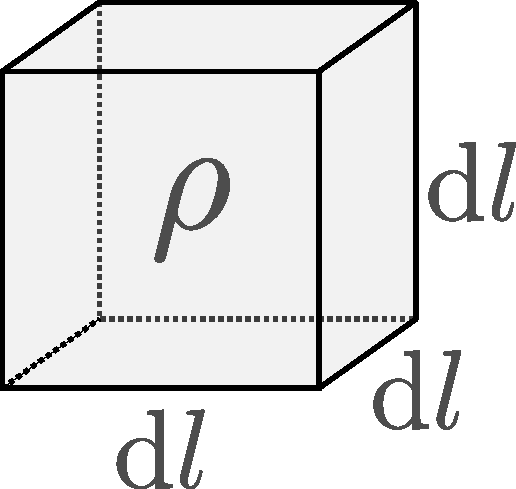
\includegraphics{../assets/2_equations/eom.pdf}
\caption{Infinitesimal box with sides of length \(\mathrm{d}l\) used to
determine the equation of motion.}
\end{figure}

The mass of the box is simply

\[\mathrm{d}m = \rho \mathrm{d} V = \rho(\mathrm{d}l)^3\]

If we consider the box is moving with the fluid, rather than being
static in space, we can write its equation of motion as
\(\mathrm{d}m\cdot\vec{a}=\vec{f}\), where \(\vec{a}\) is the
acceleration and \(\vec{f}\) are the forces acting on the box:

\[\mathrm{d}m\cdot \vec{a}=\vec{f}=\vec{f}_g + \vec{f}_P\]

where we have separated the forces into the contribution from gravity
and that from the fluid pressure. The gravitational force can be
expressed as the gradient of the gravitational potential, which in turn
must satisfy Poisson's equation,

\[\vec{f}_g=-\mathrm{d}m\nabla\Phi,\quad \nabla^2\Phi = 4\pi G \rho.\]

To compute \(\vec{f}_P\), we focus first on its component in one
cartesian direction. If our box is aligned with the \(x\) axis, then the
force of pressure will be given by the difference in pressure between
two sides, multiplied by the area of the face. This is illustrated in
the figure below, where \(P_{-x}\) and \(P_{+x}\) is the value of the
pressure at each side.

\begin{figure}
\centering
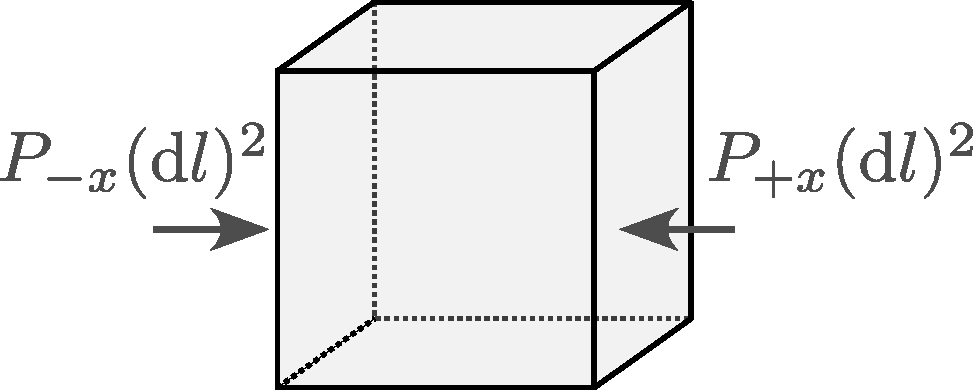
\includegraphics{../assets/2_equations/pressure.pdf}
\caption{Pressure acting on two opposite faces of the box.}
\end{figure}

The \(x\) component of the pressure force is then

\[\vec{f}_P\cdot \hat{x}=(\mathrm{d}l)^2\left(P_{-x}-P_{+x}\right)\]
\[= (\mathrm{d}l)^3 \left(\frac{\partial P}{\partial x}\right)_t,\]

where the partial derivative is taken at constant time. Repeating this
in all directions we find

\[\vec{f}_P = -\mathrm{d} V\left(\left(\frac{\partial P}{\partial x}\right)_t, \left(\frac{\partial P}{\partial y}\right)_t, \left(\frac{\partial P}{\partial z}\right)_t\right)=-\mathrm{d}V \nabla P,\]

which gives us the equation of motion

\[\vec{a}=-\nabla\Phi -\frac{\nabla P}{\rho}.\]

If we consider spherical symmetry, we find that

\[\boxed{a_r = -\frac{G m(r)}{r^2}-\frac{1}{\rho}\frac{\partial P}{\partial r},}\]

where \(m(r)\) is the mass contained inside the radius \(r\) and we have
used that in spherical symmetry \(\nabla \Phi = Gm(r)/r^2\).

\hypertarget{energy-equation}{%
\subsection{Energy equation}\label{energy-equation}}

We consider the second law of thermodynamics,

\[T\frac{\mathrm{d} s}{\mathrm{d} t}=\frac{\mathrm{d} q}{\mathrm{d} t},\]

where \(s\) is the specific entropy (meaning, per unit mass) and
\(dq/dt\) is the head added per unit mass and per unit time. Here we are
also distinguishing between a co-moving time derivative
(\(\mathrm{d}/\mathrm{d}t\)) and a time derivative fixed in space
(\(\partial /\partial t\)). In three dimensions these two operators are
related via

\[\frac{\mathrm{d}}{\mathrm{d} t} = \frac{\partial}{\partial t} + v\cdot\nabla.\]

If we have an energy flux \(\vec{F}\) going through the fluid, our mass
element \(\mathrm{d}m\) can have energy deposited onto it if \(\vec{F}\)
is not constant in space. To determine this, we apply a similar
reasoning to what we did in the previous section, considering first the
energy that flows through two sides of the box in the \(x\) direction.
The energy being deposited in each side of the box corresponds to the
flux times the area, as illustrated below where \(F_{x,-x}\) and
\(F_{x,+x}\) represent the flux at each of the faces.

\begin{figure}
\centering
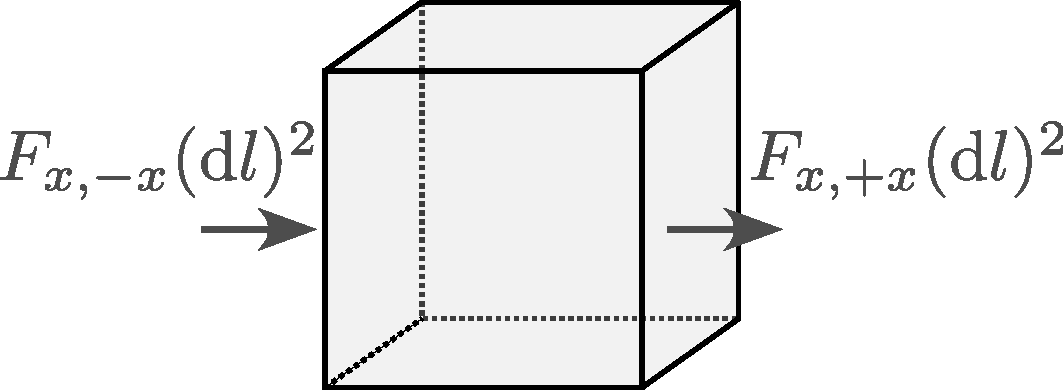
\includegraphics{../assets/2_equations/flux.pdf}
\caption{Flux crossing the cube along one axis.}
\end{figure}

The heat deposited by radiation (per unit time and mass) in the \(x\)
direction is then

\[\frac{\mathrm{d} q}{\mathrm{d} t}=\frac{(\mathrm{d}l)^2}{\mathrm{d}m}\left(F_{x,-x}-F_{x,+x}\right)\]
\[=-\frac{(\mathrm{d}l)^3}{\mathrm{d}m}\left(\frac{\partial F_x}{\partial x}\right)_t=-\frac{1}{\rho}\left(\frac{\partial F_x}{\partial x}\right)_t\]

Combining contributions from all directions we have

\[\frac{\mathrm{d} q}{\mathrm{d} t}=-\frac{1}{\rho}\left[\left(\frac{\partial F_x}{\partial x}\right)_t+\left(\frac{\partial F_y}{\partial y}\right)_t + \left(\frac{\partial F_z}{\partial z}\right)_t\right]=-\frac{\nabla\cdot \vec{F}}{\rho}\]
\[\rightarrow T\frac{\mathrm{d} s}{\mathrm{d} t} = -\frac{\nabla\cdot \vec{F}}{\rho}.\]

And if we consider spherical symmetry the result is

\[T\left(\frac{\partial s}{\partial t}\right)_m=-\frac{1}{\rho}\cdot\frac{1}{r^2}\left(\frac{\partial(r^2 F_r)}{\partial r}\right)_t,\]

where the comoving time derivative in 1D corresponds to taking the time
derivative at a fixed mass coordinate. Generally one uses the luminosity
\(L=4\pi r^2 F_r\) rather than the flux, which gives us

\[T\left(\frac{\partial s}{\partial t}\right)_m=-\frac{1}{4\pi \rho r^2}\left(\frac{\partial L}{\partial r}\right)_t.\]

In practice, we don't only have heat deposited by variations in the
flux, but also locally through nuclear reactions. If
\(\varepsilon_\mathrm{nuc}\) is the energy deposited per unit mass and
time, then we have

\[\left(\frac{\partial q}{\partial t}\right)_m=-\frac{\nabla \cdot \vec{F}}{\rho}+\varepsilon_\mathrm{nuc}\]
\[\rightarrow \boxed{T\left(\frac{\partial s}{\partial t}\right)_m=-\frac{1}{4\pi \rho r^2}\left(\frac{\partial L}{\partial r}\right)_t + \varepsilon_\mathrm{nuc}}\]

\hypertarget{continuity-equation}{%
\subsection{Continuity equation}\label{continuity-equation}}

The continuity equation describes how the density evolves as a function
of time. To obtain this equation we can think again about our box with
sides \(\mathrm{d}l\), but this time we will consider the box to be
static in space rather than comoving with the fluid. In this case we
have that the volume \(\mathrm{d}V\) of the box remains constant, but
not its mass \(\mathrm{d}m\). In particular,

\[\mathrm{dm}=(dl)^3\rho \rightarrow \frac{\partial \rho}{\partial t}=\frac{1}{\mathrm{dV}}\frac{\partial(\mathrm{d}m)}{\partial t}.\]

The image below shows how, during an amount of time \(\mathrm{d}t\),
material would flow from the two sides of the box in the x-direction.

\begin{figure}
\centering
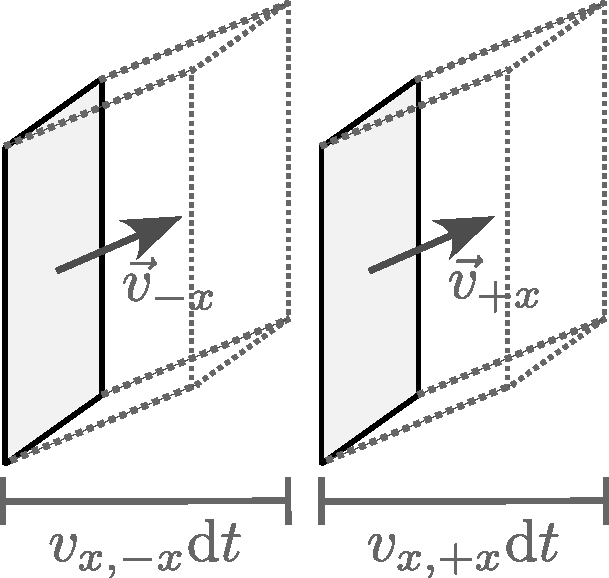
\includegraphics{../assets/2_equations/continuity.pdf}
\caption{Material crossing two opposite faces of a box (considered fixed
relative to the velocity field).}
\end{figure}

Material coming from the \(-x\) direction would fill a region of volume
\((\mathrm{d}l)^2v_{x,-x}\mathrm{d}t\), from which the total mass
flowing is obtained by mutiplying by the density at the face. The
corresponding change in mass at each face is then

\[\mathrm{d}(\mathrm{d}m)_{-x}=(\mathrm{d}l)^2 v_{x,-x}\rho_{-x}\mathrm{d}t,\]
\[\mathrm{d}(\mathrm{d}m)_{+x}=(\mathrm{d}l)^2 v_{x,+x}\rho_{+x}\mathrm{d}t.\]

We can then proceed in the same way as we did in the previous section to
compute \(\partial (\mathrm{d} m)/\partial t\), which will give us

\[\boxed{\frac{\partial \rho}{\partial t}=-\nabla \cdot (\rho \vec{v})},\]

which is known as the continuity equation. If we consider spherical
symmetry we find that

\[\left(\frac{\partial \rho}{\partial t}\right)_r=-\frac{1}{r^2}\frac{\partial}{\partial r}\left(r^2 \rho v_r\right).\tag{1.1}\]

Note that the time derivative is taken at fixed radius rather than at
fixed mass coordinate, as we were considering how properties change at a
fixed location in space rather following a comoving mass element.

\hypertarget{eularian-versus-lagrangian-description}{%
\subsection{Eularian versus Lagrangian
description}\label{eularian-versus-lagrangian-description}}

In practice, we often use the mass coordinate \(m(r)\) as a variable
instead of \(r\),

\[m(r,t)=\int_0^r 4\pi r'^{2} \rho(r',t) \mathrm{d}r'\tag{1.2}\]
\[\rightarrow \left(\frac{\partial m}{\partial r}\right)_t = 4\pi r^2\rho\quad\mathrm{or}\quad\left(\frac{\partial r}{\partial m}\right)_t = \frac{1}{4\pi r^2\rho}\tag{1.3}.\]

The change of \(m(r,t)\) with respect to time is given by the mass flux
over a shell at fixed radius \(r\),

\[\left(\frac{\partial m}{\partial t}\right)_r = -4\pi r^2 \rho v_r. \tag{1.4}\]

\begin{table*}
  \begin{center}
  \begin{tabular}{l|cc}
    & Eularian & Lagrangian \\
    \hline
    Independent variable & \(m=m(r)\) & \(r=r(m)\) \\
    Continuity equation &
    \(\displaystyle\frac{\partial m}{\partial r}=4\pi r^2\rho\) &
    \(\displaystyle{\frac{\partial r}{\partial m}}=\frac{1}{4\pi r^2 \rho}\) \\
    Equation of motion &
    \(\displaystyle a_r = -\frac{Gm}{r^2} - \frac{1}{\rho}\frac{\partial P}{\partial r}\)
    &
    \(\displaystyle a_r = -\frac{Gm}{r^2} - 4\pi r^2\frac{\partial P}{\partial m}\) \\
    Energy equation &
    \(\displaystyle T\frac{\partial s}{\partial t}=-\frac{1}{4\pi r^2 \rho}\frac{\partial L}{\partial r}+\varepsilon_\mathrm{nuc}\)
    &
    \(\displaystyle T\frac{\partial s}{\partial t}=-\frac{\partial L}{\partial m}+\varepsilon_\mathrm{nuc}\)
  \end{tabular}
\end{center}
\end{table*}

One can combine Equations \((1.2)\), \((1.2)\) and \((1.3)\) to obtain
the equation of continuity under the assumption of radial symmetry
(Equation \((1.1)\)). Owing to this, Equation \((1.3)\) is normally
referred to as the continuity equation in stellar astrophysics. We will
generally be working under the assumption of hydrostatic equilibrium, in
which case there is no difference between time derivatives at constant
radius or mass coordinate. Derivatives with respect to radius and mass
coordinate also are always taken at fixed time. Because of this we will
drop the specification of which quantity is taken to be fixed from the
partial derivatives, as they can be identified from the context.

We then have two different forms for the equations of stellar structure
and evolution, which depend on whether we use \(r\) or \(m\) as the
independent spatial variable. If \(r\) is the independent variable then
the equations are in ``Eularian'' form, while using \(m\) as independent
variable is the ``Lagrangian'' form. The equation of continuity
\((1.3)\) can be used to switch between both formulations, and these are
summarized in the table below (note that for the energy equation we are
using a time derivative at fixed mass in both formulations).

%\begin{longtable}[]{@{}
%  >{\raggedright\arraybackslash}p{(\columnwidth - 4\tabcolsep) * \real{0.2174}}
%  >{\raggedright\arraybackslash}p{(\columnwidth - 4\tabcolsep) * \real{0.3478}}
%  >{\raggedright\arraybackslash}p{(\columnwidth - 4\tabcolsep) * \real{0.4348}}@{}}
%\toprule()
%\begin{minipage}[b]{\linewidth}\raggedright
%\end{minipage} & \begin{minipage}[b]{\linewidth}\raggedright
%Eularian
%\end{minipage} & \begin{minipage}[b]{\linewidth}\raggedright
%Lagrangian
%\end{minipage} \\
%\midrule()
%\endhead
%Independent variable & \(m=m(r)\) & \(r=r(m)\) \\
%Continuity equation &
%\(\displaystyle\frac{\partial m}{\partial r}=4\pi r^2\rho\) &
%\(\displaystyle{\frac{\partial r}{\partial m}}=\frac{1}{4\pi r^2 \rho}\) \\
%Equation of motion &
%\(\displaystyle a_r = -\frac{Gm}{r^2} - \frac{1}{\rho}\frac{\partial P}{\partial r}\)
%&
%\(\displaystyle a_r = -\frac{Gm}{r^2} - 4\pi r^2\frac{\partial P}{\partial m}\) \\
%Energy equation &
%\(\displaystyle T\frac{\partial s}{\partial t}=-\frac{1}{4\pi r^2 \rho}\frac{\partial L}{\partial r}+\varepsilon_\mathrm{nuc}\)
%&
%\(\displaystyle T\frac{\partial s}{\partial t}=-\frac{\partial L}{\partial m}+\varepsilon_\mathrm{nuc}\) \\
%\bottomrule()
%\end{longtable}

Now we can ask, can we actually solve these equations? On top of initial
conditions, we need boundary conditions (BCs) for each equation
containing a spatial derivative (as these will result in an integration
constant). Two general BCs can be set at the center of the star,

\[r(m=0)=0,\quad L(m=0)=0.\]

We need one additional boundary condition, which can be set at the
surface. In regular applications, one uses a definition of a
photosphere, where the density and pressure are finite and most photons
freely travel to infinity. For analytical purposes it is better to
approximate the surface as the place where pressure vanishes,

\[P(m=M)=0,\]

where \(M\) is the total mass of the star. The two conditions at the
core are very general, while we will refine the one at the surface later
on in the course.

We can then count the number of unknowns against the number of
differential equations. We have not considered composition yet, but for
each element we consider, we will have one equation describing its time
derivative. Using a Lagrangian formulation we have the following
unknowns:

\begin{itemize}
\tightlist
\item
  The radius \(r(m,t)\)
\item
  The density \(\rho(m,t)\)
\item
  The pressure \(P(m,t)\)
\item
  The specific entropy \(s(m,t)\)
\item
  The temperature \(T(m,t)\)
\item
  The luminosity \(L(m,t)\)
\item
  And the rate of nuclear energy generation rate
  \(\varepsilon_\mathrm{nuc}(m,T)\)
\end{itemize}

This is a total of 7 unknown variables, with only 3 differential
equations! This conundrum will be solved in the following way:

\begin{itemize}
\tightlist
\item
  \(\rho\), \(P\), \(s\) and \(T\): An equation of state (EOS) of the
  fluid will give us two of these properties by specifying any of the
  other two (as well as the composition). This reduces the number of
  unknown properties by 2.
\item
  \(L\): This will come from our study of energy transport, which will
  give us an equation for \(L\) in terms of all other local properties
  such as the temperature gradient.
\item
  \(\varepsilon_\mathrm{nuc}\): This is a microphysical property that
  depends on local conditions such as temperature, density, and
  composition. We will see how it is computed when we study nuclear
  reactions.
\end{itemize}

\hypertarget{virial-theorem}{%
\subsection{Virial theorem}\label{virial-theorem}}

Consider the Lagrangian form of the equation of motion, in the case
where gravity and the pressure gradient are perfectly balanced such that
there is no acceleration. Then one obtains the equation of hydrostatic
equilibrium:

\[\boxed{\frac{\partial P}{\partial m}=-\frac{Gm}{4\pi r^4}.}\]

A very useful expression, known as the virial theorem, can be derived by
multiplying both sides by \(4\pi r^3\) and integrating over mass,

\[\int_0^M 4\pi r^2 \frac{\partial P}{\partial m}\mathrm{d}m=\int_0^M -\frac{Gm}{r}\mathrm{d}m\]

The right hand term is the gravitational potential energy, \(E_g\),
which corresponds to assembling the star by succesively bringing mass
elements \(\mathrm{d}m\) from infinity. The left hand side can be
rewritten using integration by parts:

\[\int_0^M 4\pi r^2 \frac{\partial P}{\partial m}\mathrm{d}m = \left.(4\pi r^2 P)\right|_{m=0}^{m=M}-\int 12\pi r^2 \frac{\partial r}{\partial m}P \mathrm{d}m.\]

The first term on the right hand side vanishes from the boundary
conditions, and using the continuity equation we have

\[\int 4\pi r^2 \frac{\partial P}{\partial m}\mathrm{d}m = -3\int_0^M\frac{P}{\rho}\mathrm{d}m,\]

which gives us the virial theorem

\[\boxed{E_g = -3\int_0^M\frac{P}{\rho}\mathrm{d}m}\tag{1.5}\]

To see what this implies, let's consider the very simple case of a
monoatomic gas:

\[P=nk_\mathrm{B}T,\quad n=\frac{\rho}{m_g},\tag{1.6}\]

where \(k_\mathrm{B}\) is Boltzmann's constant and \(m_g\) is the mass
of the individual gas particles. This is very simplified as it does not
account for electrons in an ionized gas, but this will be generalized in
later classes. For the monoatomic ideal gas the energy per particle is

\[e=\frac{3}{2}k_\mathrm{B}T,\]

from which we can compute the specific (meaning, per unit mass) internal
energy of the gas,

\[u=\frac{e}{m_g}=\frac{3}{2}\frac{k_\mathrm{B}T}{m_g}.\tag{1.7}\]

Plugging \((1.7)\) and \((1.6)\) into \((1.5)\) we find

\[E_g = -2\int_0^M u \mathrm{d}m=-2E_i,\]

where \(E_i\) is the internal energy of the gas. The total energy of the
gas can be determined by adding up the potential and gravitational
energies, which combined with the previous equation results in

\[E=E_g+E_i=-E_i.\]

From this we see that the total energy is negative (as expected for a
bound star) and that as a star loses (for instance, due to radiation at
their surface), its internal energy increases. This implies that a star
will often increase its temperature as a consequence of mass loss! Often
this is referred to as stars having a negative heat capacity.

\hypertarget{lane-emden-equation}{%
\subsection{Lane-Emden equation}\label{lane-emden-equation}}

Consider the continuity and hydrostatic equilibrium equations in their
Eularian form,

\[\frac{\partial m}{\partial r}=4\pi r^2 \rho,\quad \frac{\partial P}{\partial r}=-\frac{Gm\rho}{r^2}.\]

It could be possible to find solutions to these equations if there was a
simple relationship of the form \(P=P(\rho)\) (meaning, temperature
independent), such that we only have as unknowns \(\rho(r)\) and
\(m(r)\). As it turns out an important particular case is that of a so
called polytropic equation of state,

\[P=K\rho^\gamma,\]

where \(K\) and \(\gamma\) are constant. Depending on the relevant
equation of state that describes a star at a given stage, we will see
both cases where \(K\) is a function of fundamental constants that is
independent of a specific star, as well as cases where \(K\) can vary
during the evolution of a star. Rather than using the exponent
\(\gamma\), it is common to use the polytropic index \(n\), with

\[P=K\rho^{1+1/n}.\]

We can combine the equation of hydrostatic equilibrium with the equation
of continuity to obtain a single second order differential equation as
follows:

\[\left.\frac{\partial P}{\partial r}=-\frac{Gm\rho}{r^2}\quad\right/ \frac{r^2}{\rho}\cdot\]
\[\left.\frac{r^2}{\rho}\frac{\partial P}{\partial r}=-Gm\quad\right/ \frac{\partial}{\partial r}\cdot\]
\[\frac{\partial}{\partial r}\left(\frac{r^2}{\rho}\frac{\partial P}{\partial r}\right)=-G\frac{\partial m}{\partial r}=-4\pi G \rho r^2.\tag{1.8}\]

If we have a polytropic relationship between density and pressure, then
this is just a second order differential equation for \(\rho(r)\), and
we can obtain a solution for it if we have two boundary conditions. A
useful dimensionless form of this equation can be obtained if we define
a new variable \(z\) instead of \(r\) from

\[r=r_n z,\qquad r_n \equiv \sqrt{\frac{(n+1)P_c}{4\pi G\rho_c^2}},\]

and we define a function \(w(z)\) such that

\[\rho = \rho_c \left[w(z)\right]^n\rightarrow P=P_c\left[w(z)\right]^{n+1},\]

where \(\rho_c\) and \(P_c\) are the central density and pressure. Using
\(z\) and \(w(z)\) to replace \(r\), \(\rho\) and \(P\) in Equation
(1.8), one obtains the Lane-Emden equation:

\[\frac{1}{z^2}\frac{\mathrm{d}}{\mathrm{d} z}\left(z^2\frac{\mathrm{d}w}{\mathrm{d}z}\right)=-w^n.\]

We need two boundary conditions, one of them clearly being \(w(0)=1\) as
we require the central density and pressure to be \(\rho_c\) and \(P_c\)
respectively. The second boundary condition can be determined from a
restriction on the central temperature gradient. Since near the core the
mass is given by \(m\simeq 4\pi r^3 \rho_c/3\), the equation of
hydrostatic equilibrium implies that
\((\partial P/\partial r)|_{r=0}=0\) which in turn implies that
\(w'|_{\xi=0}=0\). With these two boundary conditions the Lane-Emden
equation has a unique solution for each \(n\), and using our definition
of the stellar surface as \(P(R)=0\), the surface is determined by the
first value \(\xi_1\) for which \(w(\xi_1)=0\). As we consider different
equations of state that can be approximated as polytropes, the
Lane-Emden equation will be a useful source of insight to determine how
different properties of the star (such as their mass and radius) relate
to each other.

\hypertarget{the-energy-equation-and-the-equation-of-state-eos}{%
\section{The energy equation and the equation of state
(EOS)}\label{the-energy-equation-and-the-equation-of-state-eos}}


\hypertarget{energy-equation-and-global-energetics}{%
\subsection{Energy equation and global
energetics}\label{energy-equation-and-global-energetics}}

Let's consider the energy equation in its Lagragian form:

\[T\frac{\partial s}{\partial t}=\frac{\partial q}{\partial t}=\varepsilon_\mathrm{nuc}-\frac{\partial L}{\partial m}.\tag{2.1}\]

We can rewrite this using the first law of thermodynamics, which states
that

\[\mathrm{d}U = \mathrm{d}Q - P\mathrm{d}V.\]

This form of the first law describes a body of volume \(V\) with a
surface pressure \(P\) and total energy \(U\), to which an amount of
heat \(\mathrm{d}Q\) is deposited. We want to work with local properties
of our gas, for which we make use of specific (meaning, per unit mass)
quantities,

\[\mathrm{d}u=\mathrm{d}q -P \mathrm{d}v, \quad v\equiv \frac{1}{\rho},\]

where \(v\) is the volume per unit mass. More commonly \(v\) is reserved
for the velocity, but in this chapter we reserve it exclusively for the
specific volume. The energy equation (2.1) can then be rewritten as

\[\frac{\partial u}{\partial t}+P\frac{\partial v}{\partial t}=\varepsilon_\mathrm{nuc}-\frac{\partial L}{\partial m}.\]

To describe global properties of the star we can integrate this equation
over the total mass of the star,

\[\int_0^M\left[\frac{\partial u}{\partial t}+P\frac{\partial v}{\partial t}\right]\mathrm{d}m=\int_0^M\left[\varepsilon_\mathrm{nuc}-\frac{\partial L}{\partial m}\right]\mathrm{d}m.\tag{2.2}\]

Integrating \(\varepsilon_\mathrm{nuc}\) gives us the total nuclear
energy generation rate in the star, to which we refer as
\(L_\mathrm{nuc}\). We also have that

\[\int_0^M\frac{\partial u}{\partial t}\mathrm{d}m=\frac{\partial}{\partial t}\int_0^M u\mathrm{d}m = \dot{E}_i,\]

where we recall that \(E_i\) is the total internal energy of the gas.
Using this Equation (2.2) becomes

\[\dot{E}_i+\int_0^M P\frac{\partial v}{\partial t}\mathrm{d}m=L_\mathrm{nuc}-L_\mathrm{surf}+L(0),\]

where \(L_\mathrm{surf}=L(m=M)\) is the luminosity at the stellar
surface. Using the central boundary condition on the luminosity we get
that

\[\dot{E}_i-\int_0^M P\frac{\partial v}{\partial t}\mathrm{d}m = L_\mathrm{nuc}-L_\mathrm{surf}.\]

The right hand side of this equation is equal to the energy injected
onto the star minus the energy radiated away from its surface. We then
expect the left hand side of the equation to correspond to the rate of
change of the total energy \(E=E_i+E_g\). For this to be true, then we
require that

\[\dot{E}_g = \int_0^MP\frac{\partial v}{\partial t}\mathrm{d}m. \tag{2.4}\]

We take Equation \((2.4)\) as a consequence of the energy equation, but
instead, let's verify that it is correct in terms of the definition of
\(E_g\) and the equation of hydrostatic equilibrium. First, it is
straightforward to relate \(\dot{v}\) to \(\dot{\rho}\):

\[\frac{\partial v}{\partial t}=\frac{\partial}{\partial t}\left(\frac{1}{\rho}\right)=-\frac{\dot{\rho}}{\rho^2}\]
\[\rightarrow \int_0^M P\frac{\partial v}{\partial t}\mathrm{d}m = -\int_0^M \frac{P\dot{\rho}}{\rho^2}\mathrm{d}m.\tag{2.5}\]

We can also obtain \(\dot{E}_g\) from the virial theorem:

\[E_g=-3\int_0^M\frac{P}{\rho}\mathrm{d}m\]
\[\rightarrow\dot{E}_g=-3\int_0^M\frac{\dot{P}}{\rho}\mathrm{d}m + 3\int_0^M\frac{P\dot{\rho}}{\rho^2}\mathrm{d}m \tag{2.6}\]

The first integral on the right hand side can be obtained from the
equation of hydrostatic equilibrium,

\[\left.\frac{\partial P}{\partial m}=-\frac{Gm}{4\pi r^4}\quad\right/\frac{\partial}{\partial t}\cdot\]
\[\left.\frac{\partial \dot{P}}{\partial m}=4\frac{Gm}{4\pi r^4}\frac{\dot{r}}{r}\quad\right/4\pi r^3\cdot\]
\[\left.4\pi r^3 \frac{\partial \dot{P}}{\partial m}=4\frac{Gm}{r}\frac{\dot{r}}{r}\quad\right/\int_0^M(\;)\mathrm{d}m\]
\[\int_0^M 4\pi r^3 \frac{\partial \dot{P}}{\partial m}\mathrm{d}m=4\int_0^M\frac{Gm}{r}\frac{\dot{r}}{r}\mathrm{d}m.\tag{2.7}\]

From the definition of \(E_g\) we have

\[E_g=-\int_0^M\frac{Gm}{r}\mathrm{d}m\]
\[\rightarrow \dot{E}_g=\int_0^M \frac{Gm}{r}\frac{\dot{r}}{r}\mathrm{d}m.\]

Replacing this in Equation \((2.7)\) and integrating the left hand side
by parts gives

\[\left.\left(4\pi r^3 \dot{P}\right)\right|_0^M-3\int_0^M 4\pi r^2 \frac{\partial r}{\partial m}\dot{P}\mathrm{d}m=4\dot{E}_g,\]

where the first term is zero due to the boundary conditions, and using
the equation of continuity to replace \(\partial r/\partial m\) results
in

\[-3\int_0^M\frac{\dot{P}}{\rho}\mathrm{d}m=4\dot{E}_g.\]

Replacing this in Equation \((2.6)\) one obtains

\[\dot{E}_g=-\int_0^M \frac{P\dot{\rho}}{r^2}\mathrm{d}m,\]

which combined with Equation \((2.5)\) shows that indeed Equation
\((2.4)\) is correct. This means that Equation \((2.3)\) is equivalent
to

\[L_\mathrm{nuc}-L_\mathrm{surf}=\dot{E}_i+\dot{E}_g = \dot{E},\]

which is what we expect in terms of the evolution of the total energy
and its sinks and sources.

\hypertarget{eos-definitions}{%
\subsection{EOS definitions}\label{eos-definitions}}

We want to express the energy equation \((2.1)\) in terms of something
other than entropy. By virtue of the first law of thermodynamics, we
already showed that

\[\frac{\partial u}{\partial t}+P\frac{\partial v}{\partial t}=\varepsilon_\mathrm{nuc}-\frac{\partial L}{\partial m}.\tag{2.8}\]

In general, the local state of the fluid is determined by a pair of
properties, such as pressure and temperature (and also composition, but
for now we ignore changes in it). The version of the energy equation
above uses internal energy and density (in terms of the specific
volume), but we could use any other pair of independent thermodynamic
properties of the fluid. To write this in a form commonly used in
stellar evolution theory, we will switch it to use pressure and
temperature.

Before we do so, we will first define some terms associated to an
equation of state. If we consider an EOS of the form

\[\rho=\rho(P,T),\]

then changes in density are related to changes in pressure and
temperature as

\[\mathrm{d}\rho = \left(\frac{\partial \rho}{\partial P}\right)_T\mathrm{d}P + \left(\frac{\partial\rho}{\partial T}\right)_P\mathrm{d}T. \tag{2.9}\]

The partial derivatives are commonly expressed in terms of logarithmic
derivatives,

\[\left(\frac{\partial \rho}{\partial P}\right)_T=\frac{\mathrm{d}\rho}{\mathrm{d}\ln \rho}\left(\frac{\partial \ln \rho}{\partial \ln P}\right)_T\frac{\mathrm{d}\ln P}{\mathrm{d}P}=\frac{\rho}{P}\left(\frac{\partial \ln \rho}{\partial \ln P}\right)_T.\]

If we define

\[\alpha\equiv \left(\frac{\partial \ln \rho}{\partial \ln P}\right)_T, \quad \delta=-\left(\frac{\partial\ln\rho}{\partial\ln T}\right)_P,\]

then Equation (2.9) turns into

\[\frac{\mathrm{d}\rho}{\rho}=\alpha\frac{\mathrm{d}P}{P}-\delta \frac{\mathrm{d}T}{T}.\]

If we know the the form \(\rho=\rho(P,T)\) of the EOS, \(\alpha\) and
\(\delta\) can be derived from it. Two other quantities that will be
useful are the heat capacities. The heat capacity at constant pressure
is:

\[c_P\equiv \left(\frac{\partial q}{\partial T}\right)_P=\left(\frac{\partial u}{\partial T}\right)_P+P\left(\frac{\partial v}{\partial T}\right)_P,\]

and similarly, we have the specific heat at constant volume,

\[c_v\equiv \left(\frac{\partial q}{\partial T}\right)_v=\left(\frac{\partial u}{\partial T}\right)_v.\]

\hypertarget{rewriting-the-energy-equation}{%
\subsection{Rewriting the energy
equation}\label{rewriting-the-energy-equation}}

We aim to write the energy equation (2.8) in terms of the pressure and
temperature. For this we have that

\[\mathrm{d}q=\mathrm{d}u+P\mathrm{d}v=A\mathrm{d}T+B\mathrm{d}P.\]

Our objective is to find \(A\) and \(B\). For this we will need two
seemingly (at first) unrelated results.

\begin{enumerate}
\def\labelenumi{\arabic{enumi}.}
\item
  Consider the relationship between \(u\), \(v\) and \(T\),

  \[\mathrm{d}u = \left(\frac{\partial u}{\partial v}\right)_T \mathrm{d}v + \left(\frac{\partial u}{\partial T}\right)_v\mathrm{d}T.\tag{2.10}\]

  We also have that

  \[\mathrm{d}s=\frac{\mathrm{d}q}{T}=\frac{1}{T}\left(\mathrm{d}u + P\mathrm{d}v\right),\]

  were after applying Equation \((2.10)\) gives us

  \[\mathrm{d}s=\frac{1}{T}\left[\left(\frac{\partial u}{\partial v}\right)_T + P\right]\mathrm{d}v + \frac{1}{T}\left(\frac{\partial u}{\partial T}\right)_v.\]

  As \(\mathrm{d}s\) is a total differential (in contrast to
  \(\mathrm{d}q\) which is an
  \href{https://en.wikipedia.org/wiki/Inexact_differential}{imperfect
  differential}) we have that

  \[\frac{\partial^2 s}{\partial T\partial v}=\frac{\partial^2 s}{\partial v\partial T}\]
  \[\rightarrow \frac{\partial}{\partial T}\left[\frac{1}{T}\left(\frac{\partial u}{\partial v}\right)_T+\frac{P}{T}\right]=\frac{1}{T}\frac{\partial^2 u}{\partial v\partial T}\]

  which after performing the derivative on the left hand side gives us
  the following relationship:

  \[\boxed{\left(\frac{\partial u}{\partial v}\right)_T=T\left(\frac{\partial P}{\partial T}\right)_v-P}\tag{2.11}\]
\item
  We will now derive a relationship between the specific heats. We start
  from \((2.10)\),

  \[\frac{\mathrm{d}u}{\mathrm{d}T}=\left(\frac{\partial u}{\partial v}\right)_T\frac{\mathrm{d} v}{\mathrm{d} T}+\left(\frac{\partial u}{\partial T}\right)_v\]
  \[\left(\frac{\partial u}{\partial T}\right)_P=\left(\frac{\partial u}{\partial v}\right)_T\left(\frac{\partial v}{\partial T}\right)_P+\left(\frac{\partial u}{\partial T}\right)_v.\]

  We use \((2.11)\) on the right hand side,

  \[\left(\frac{\partial u}{\partial T}\right)_P=\left[T\left(\frac{\partial P}{\partial T}\right)_v-P\right]\left(\frac{\partial v}{\partial T}\right)_P + \left(\frac{\partial u}{\partial T}\right)_v,\]

  and after rearranging terms we get

  \[\left(\frac{\partial u}{\partial T}\right)_P + P\left(\frac{\partial u}{\partial T}\right)_P-\left(\frac{\partial u}{\partial T}\right)_v = T\left(\frac{\partial P}{\partial T}\right)_v\left(\frac{\partial v}{\partial T}\right)_P\]
  \[c_P-c_v = T\left(\frac{\partial P}{\partial T}\right)_v\left(\frac{\partial v}{\partial T}\right)_P.\tag{2.12}\]

  We leave it as part of the exercises to show that

  \[\left(\frac{\partial P}{\partial T}\right)_v=-\frac{\left(\frac{\partial P}{\partial T}\right)_P}{\left(\frac{\partial v}{\partial P}\right)_T}=\frac{P\delta}{T\alpha}, \tag{2.13}\]

  and that

  \[T\left(\frac{\partial v}{\partial T}\right)_P=\frac{\delta}{\rho}.\]

  Using these two expressions in Equation \((2.14)\) results in

  \[\boxed{c_P-c_v = \frac{P\delta^2}{T\rho\alpha}}.\tag{2.14}\]
\end{enumerate}

We now have what we need to rewrite our energy equation. Let's start
from

\[\mathrm{d}q = \mathrm{d}u + P \mathrm{d}v.\]

Applying \((2.10)\) we get

\[\mathrm{d}q = \left(\frac{\partial u}{\partial T}\right)_v\mathrm{d}T + \left(\frac{\partial u}{\partial v}\right)_T\mathrm{d}v+P\mathrm{d}v\]
\[=\left(\frac{\partial u}{\partial T}\right)_v\mathrm{d}T+\left[\left(\frac{\partial u}{\partial v}\right)_T+P\right]\mathrm{d}v.\]

We use \((2.11)\) on the left hand side,

\[\mathrm{d}q=\left(\frac{\partial u}{\partial T}\right)_v\mathrm{d}T+T\left(\frac{\partial P}{\partial T}\right)_v\mathrm{d}v.\]

We note that \(c_v=(\partial u/\partial T)_v\) and
\(\mathrm{d}v=-\mathrm{d}\rho/\rho^2\), and use Equation \((2.13)\) on
the right hand side,

\[\mathrm{d}q = c_v\mathrm{d}T-\frac{P\delta}{\rho\alpha}\frac{\mathrm{d}\rho}{\rho}\]
\[=c_v\mathrm{d}T-\frac{P\delta}{\rho\alpha}\left(\alpha\frac{\mathrm{d}P}{P}-\delta\frac{\mathrm{d}T}{T}\right)\]
\[=\left(c_v+\frac{P\delta^2}{\rho T \alpha}\right)\mathrm{d}T-\frac{\delta}{\rho}\mathrm{d}.P\]

Using Equation \((2.14)\) we finally get what we were looking for:
\[\mathrm{d}q = c_P\mathrm{d}T-\frac{\delta}{\rho}\mathrm{d}P.\tag{2.15}\]
Using this expression we obtain the energy equation in terms of
\(\partial P/\partial t\) and \(\partial T/\partial t\),

\[\boxed{c_P\frac{\partial T}{\partial t}-\frac{\delta}{\rho}\frac{\partial P}{\partial t}=\varepsilon_\mathrm{nuc}-\frac{\partial L}{\partial m}.}\]

A very useful property of the gas is the adiabatic temperature gradient,

\[\nabla_\mathrm{ad}=\left(\frac{\partial \ln T}{\partial \ln P}\right)_\mathrm{ad},\]

where ``ad'' indicates a change at constant entropy (\(\mathrm{d}s=0\)).
Using Equation \((2.15)\) together with \(T\mathrm{d}s=\mathrm{d}q\), we
get

\[\left.\left(\frac{\partial T}{\partial P}\right)_\mathrm{ad}=-\frac{\delta}{c_P\rho}\quad\right/\frac{P}{T}\cdot\]
\[\boxed{\nabla_\mathrm{ad}=\frac{P\delta}{T\rho c_P}.}\]

We will find later on that in some cases we can approximate a star as a
ball of constant entropy, which implies

\[\nabla\equiv\frac{\partial \ln T}{\partial \ln P}=\nabla_\mathrm{ad},\]

where \(\nabla\) represents the actual temperature gradient with respect
to pressure through the star.

\hypertarget{deriving-a-pressure-from-a-distribution}{%
\subsection{Deriving a pressure from a
distribution}\label{deriving-a-pressure-from-a-distribution}}

So, once we manage to write down our EOS as \(\rho=\rho(P,T)\), and we
also determine its internal energy \(u=u(P,T)\), we can determine
\(c_P\), \(\alpha\) and \(\delta\). This gives us what we need for the
energy equation.

But how can we derive \(\rho(P,T)\) and \(u(P,T)\)? Next class we'll
work on that, considering that a gas has multiple particles with a
distribution of their velocities (and momenta). We can express the
number of particles in a volume \(\mathrm{d}V\) that have a momentum
between \(p\) and \(p+\mathrm{d}p\) as

\[N(p,p+\mathrm{d}p)=n_p\mathrm{d}p\mathrm{d}V=nf(p)\mathrm{d}p\mathrm{d}V,\]

where \(n\) is the number of particles per unit volume and \(f(p)\) is a
probability density for a particle to have a given momentum.If we can
find \(f(p)\) then we can determine macroscopic properties such as
pressure and internal energy density. For example, next week we'll show
that

\[P=\frac{1}{3}\int_0^\infty v_p p n_p\mathrm{d}p,\]

where \(v_p\) is the velocity of a particle with momentum \(p\).

\hypertarget{degenerate-equations-of-state}{%
\section{Degenerate equations of
state}\label{degenerate-equations-of-state}}

\hypertarget{deriving-u-and-p}{%
\subsection{\texorpdfstring{Deriving \(u\) and
\(P\)}{Deriving u and P}}\label{deriving-u-and-p}}

We will consider a distribution of momenta, such that the number of
particles with momentum between \(p\) and \(p+\mathrm{d}p\) in a volume
\(\mathrm{d}V\) is

\[N(p,p+\mathrm{d}p)=f(p)\mathrm{d}p\mathrm{d}V.\]

One example for \(f(p)\) is the Maxwell-Boltzmann distribution,

\[f(p)=\displaystyle n\frac{4\pi p^2}{(2\pi m k T)^{3/2}}\exp\left(-\frac{p^2}{2m k T}\right),\]

which has a maximum at

\[p_\mathrm{max}=(2m k T)^{1/2}.\]

This distribution corresponds to the momenta of particles of mass \(m\)
in an ideal monoatomic gas. In the case of an ionized gas, or a gas with
multiple ions of different type, each component follows the distribution
with their corresponding mass and particle density. For instance, for
free electrons we have

\[n_e = \displaystyle\frac{\rho}{\mu_e m_u},\]

where \(m_u\) is the atomic mass unit and \(\mu_e\) is the mean
molecular weight per electron. The quantity \(\mu_e\) can be read as the
number of atomic mass units in the fluid per electron, which means that
for pure ionized hydrogen \(\mu_e\simeq1\), while for pure ionized
helium \(\mu_e\simeq2\).

If each particle has an energy \(E(p)\), then the specific internal
energy of the gas is

\[u = \frac{1}{\rho}\int_0^\infty E(p)f(p)\mathrm{d}p,\quad E(p)=mc^2\sqrt{\displaystyle 1+\frac{p^2}{m^2c^2}},\]

as the integral gives the internal energy per unit volume, which is
turned into the specific internal energy by multiplying by the specific
volume \(\rho^{-1}\).

Computing pressure is a bit more complex. Consider a slab of area
\(\mathrm{d}\sigma\) embedded in the gas, on which particles will be
bouncing,

\begin{figure}
\centering
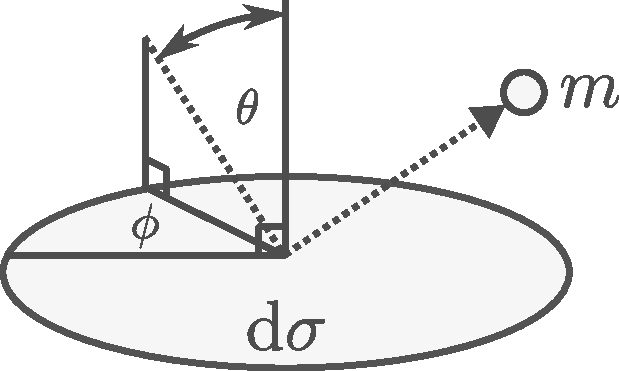
\includegraphics[width=0.4\textwidth]{../assets/4_eos2/pressure1.pdf}
\caption{Particle impacting and bouncing of an area
\(\mathrm{d}\sigma\).}
\end{figure}

A particle with momentum \(p\) colliding at an angle \(\theta\) with
respect to the normal will transfer momentum equal to

\[\Delta p = 2p\cos{\theta}. \tag{3.1}\]

The pressure corresponds to a force per unit area, and a force
corresponds to a change in momentum per unit time. This means that if we
know the rate of collisions per unit time and direction on
\(\mathrm{d}\sigma\) we can integrate over all directions to get the
pressure. Let's consider particles coming from a direction
\(\theta,\phi\), which cover a solid angle \(\mathrm{d}\vec{\Omega}\) in
the direction of their momenta \(p\) and hit the slab
\(\mathrm{d}\sigma\),

\begin{figure}
\centering
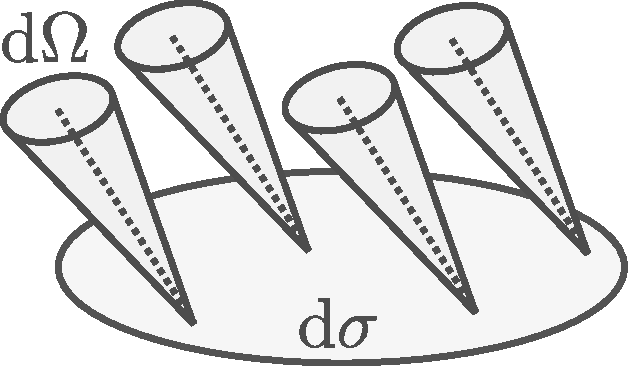
\includegraphics[width=0.4\textwidth]{../assets/4_eos2/pressure2.pdf}
\caption{Particles impacting the area \(\mathrm{d}\sigma\) from a solid
angle \(\mathrm{d}\Omega\)}
\end{figure}

As the distribution is isotropic, the number of particles with momenta
between \(p\) and \(p+\mathrm{d}p\) contained in the solid angle
\(\mathrm{d}\vec{\Omega}\) is

\[N(p,p+\mathrm{d}p,\mathrm{d}\vec{\Omega})=\frac{f(p)}{4\pi}\mathrm{d}p\mathrm{d}V\mathrm{d}\Omega.\]

next we need to know how many particles per unit time, unit momenta and
unit solid angle will cross the slab. If we consider particles with
momentum \(p\) hitting the slab at an angle \(\theta\), and take the
velocity \(v_p\) for a given momentum, then in a time \(\Delta t\) all
particles in an area \(v_p\cos\theta\mathrm{d}\sigma\Delta t\) will
cross the slab.

\begin{figure}
\centering
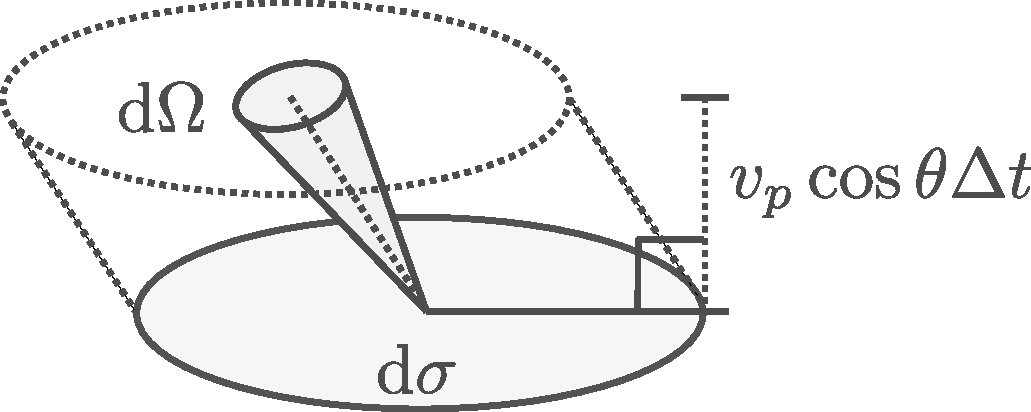
\includegraphics{../assets/4_eos2/pressure3.pdf}
\caption{Determination of particle flux impacting \(\mathrm{d}\sigma\)
from a given direction.}
\end{figure}

The number of collisions per unit time onto the slab, with momenta
between \(p\) and \(p+\mathrm{d}p\) coming from a solid angle
\(\mathrm{d}\vec{\Omega}\) is

\[r_\mathrm{coll}=\frac{f(p)}{4\pi}v_p\cos\theta\mathrm{d}\theta\mathrm{d}\sigma\mathrm{d}\rho\mathrm{d}\Omega.\]

Each of these collisions imparts a momentum \(\Delta p\) given by
equation \((3.1)\). The pressure is then obtained by integrating over
all angles in a half sphere and dividing by \(\mathrm{d}\sigma\):

\[P=\int_0^{\infty}\int_0^{2\pi}\int_0^{\pi/2} 2p\cos\theta \cdot \frac{f(p)}{4\pi}v_p\cos\theta \sin\theta \mathrm{d}\theta\mathrm{d}\phi\mathrm{d}p\]
\[P=\frac{1}{2\pi}\int_0^\infty v_p p f(p)\mathrm{d}p \int_0^{2\pi}\mathrm{d}\phi \int_0^{\pi/2}\cos^2\theta\sin\theta \mathrm{d}\theta\]
\[\boxed{P=\frac{1}{3}\int_0^\infty v_p p f(p)\mathrm{d}p,}\tag{3.2}\]

where we used
\(\mathrm{d}\Omega=\sin\theta\mathrm{d}\theta\mathrm{d}\phi\). We
already saw in the exercises last class how this expression gives the
ideal gas pressure for a Maxwell-Boltzmann distribution.

\hypertarget{pauli-exclusion-principle-and-degeneracy}{%
\subsection{Pauli exclusion principle and
degeneracy}\label{pauli-exclusion-principle-and-degeneracy}}

If we were to take a Maxwell-Boltzmann distribution and lower the
temperature towards zero, all particles would tend to zero momentum. As
electrons, protons and neutrons have half spin (ie. they are fermions),
this cannot happen as they must satisfy the Pauli exclusion principle.
If a particle has an uncertainty in momentum equal to \(\mathrm{d}^3 p\)
and an uncertainty in position \(\mathrm{d}^3 x\) then we must have

\[\mathrm{d}^3 p\mathrm{d}^3x>h^3,\]

where \(h\) is Planck's constant. Pauli's exclusion principle indicates
that only two fermions can occupy a quantum cell of 6-D volume \(h^3\).
Gases for which their properties become affected by this quantum limit
are referred to as Degenerate.

Now let's think that all particles go to their lower energy state. If we
consider a volume \(\mathrm{d}^3x\), then each particle will occupy a
momentum space

\[\mathrm{d}^3p=\frac{h^3}{2\mathrm{d}^3 x}.\]

As they go to the lowest possible energy states, we can think they fill
a sphere in momentum space up to a value \(p_\mathrm{F}\), known as the
Fermi momentum:

\begin{figure}
\centering
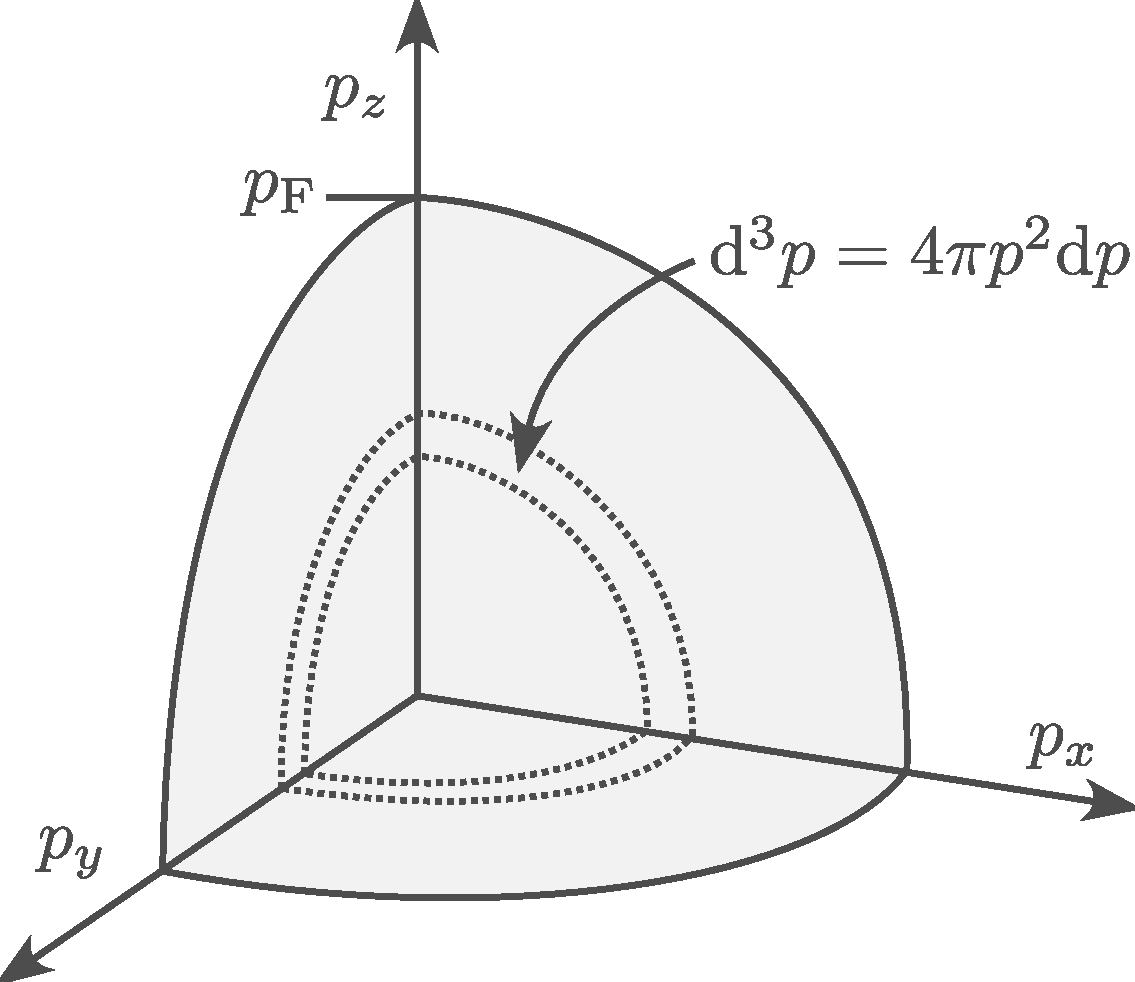
\includegraphics{../assets/4_eos2/momentum.pdf}
\caption{Distribution of particle momentum filling all lower energy
states up to the Fermi momentum.}
\end{figure}

The volume in momentum is simply

\[\int_0^p 4\pi p^2 \mathrm{d} p = \frac{4\pi}{3}p_\mathrm{F}^3.\]

Since we know each cell occupies a 3-D momentum-space volume
\(h^3/(2\mathrm{d}^3x)\), the number of particles in \(\mathrm{d}^3x\)
should be:

\[N=n\mathrm{d}^3x = \frac{\left(\displaystyle \frac{4\pi}{3}p_\mathrm{F}^3\right)}{\displaystyle \left(\frac{h^3}{2\mathrm{d}^3x}\right)}=\frac{8\pi}{3h^3}p_\mathrm{F}^3 \mathrm{d}^3 x\]
\[\rightarrow n=\frac{8\pi}{3h^3}p_\mathrm{F}^3.\]

This expression allows us to compute the Fermi momentum if we know the
particle density of the medium, meaning that for a given density, we
know the radius in momentum space that would be occupied by particles if
the sink towards the lowest energy state allowable by quantum mechanics.

So what is \(f(p)\)? Between momenta \(p\) and \(p+\mathrm{d}p\) we have
a volume in momentum equal to
\[V_\mathrm{p}(p,p+\mathrm{d}p)=4\pi p^2\mathrm{d}p.\] The number of
particles in this momentum shell within the volume \(\mathrm{d}^3 x\) is

\[N(p,p+\mathrm{d}p)=\frac{4\pi p^2 \mathrm{d}p}{\displaystyle\left(\frac{h^3}{2\mathrm{d}^3 x}\right)},\]
which from the definition of \(f(p)\) means that \[\boxed{f(p)=
\begin{cases}
\displaystyle \frac{8\pi}{h^3}p^2 & p<p_\mathrm{F} \\
0 & p>p_\mathrm{F}.
\end{cases}}\tag{3.3}
\]

So how does this compare to a Maxwell-Boltzmann distribution? The image
below (source to produce this figure available
\href{assets/4_eos2/MB_versus_degenerate.jl}{here}) shows the Maxwell
Boltzmann distribution of electron momenta for different temperatures at
the mass density of the solar core (\(\sim 150\;\mathrm{g\,cm}^{-3}\)).
The hydrogen mass fraction at the solar core is \(X\simeq 0.35\), and
the electron number density can be determined under the assumption of
full ionization using the approximation \(\mu_e=2/(1+X)\).

\begin{figure}
\centering
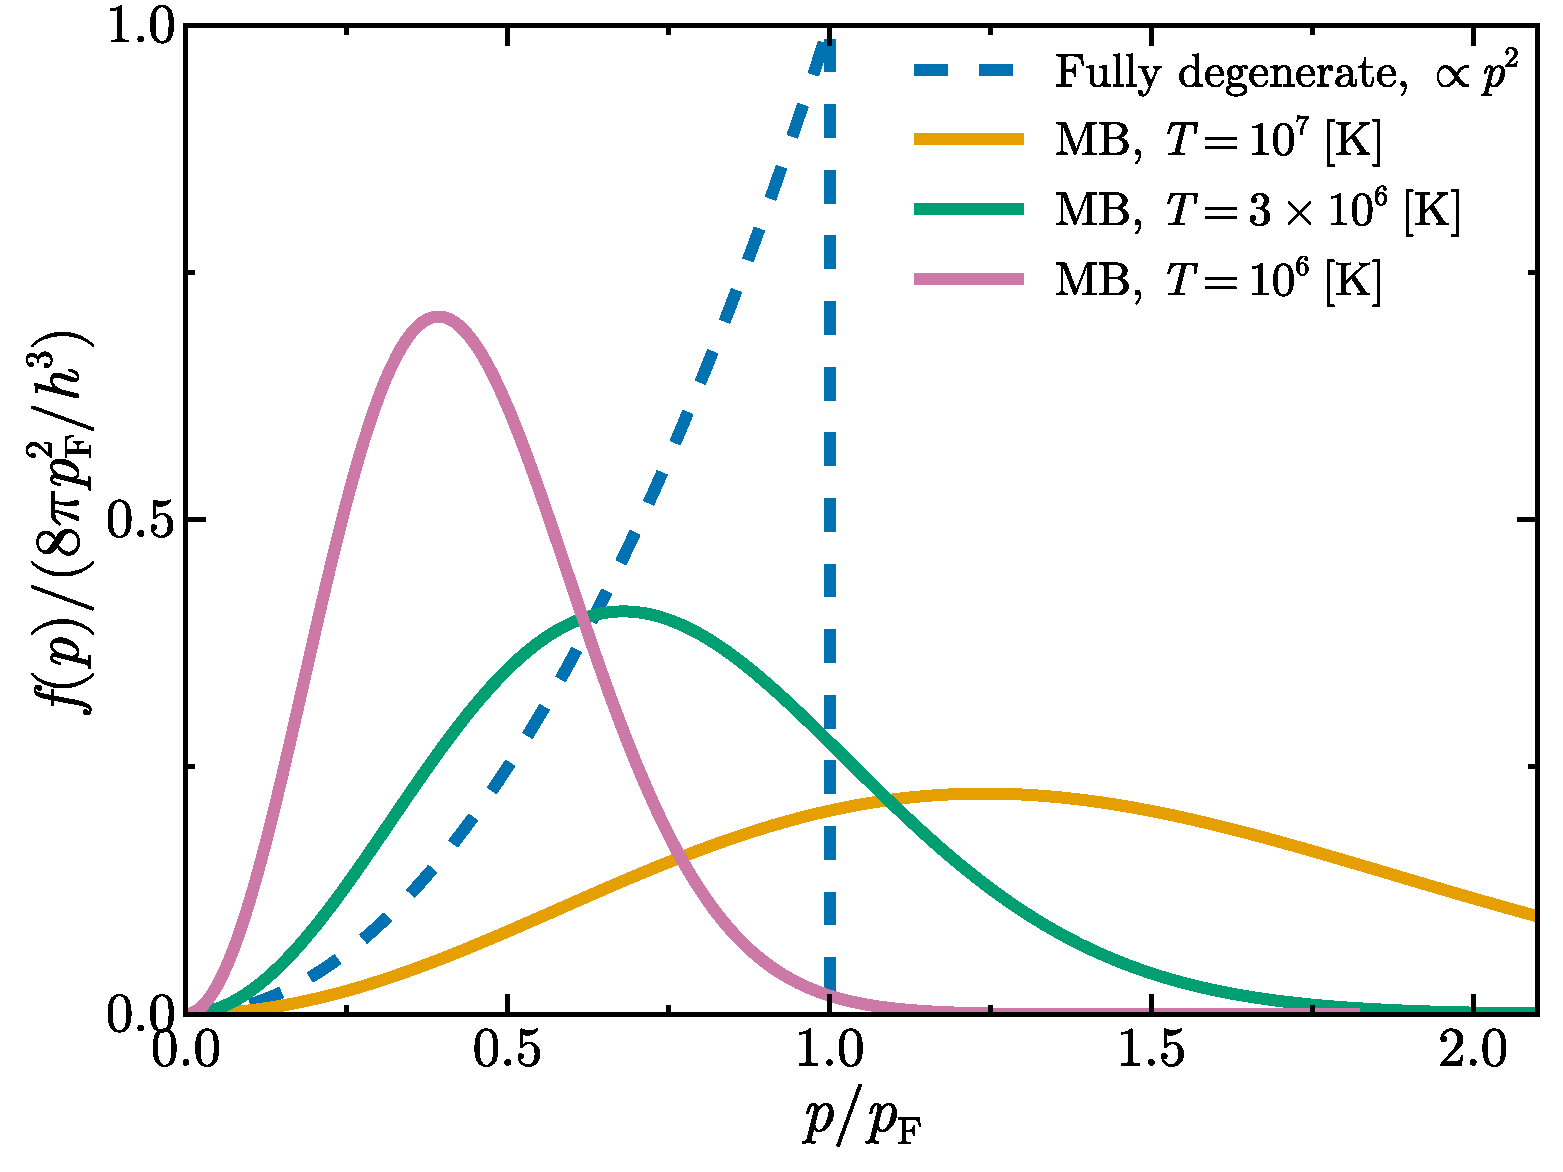
\includegraphics{../assets/4_eos2/degeneracy.pdf}
\caption{Degeneracy at solar core}
\end{figure}

The temperature at the core of the Sun is
\(\sim 1.5\times 10^7\,\mathrm{K}\), and we see that at the conditions
of the solar center a Maxwell-Boltzmann distribution does not violate
the Pauli exclusion principle. However, this is not the case as the
temperature is lowered, and we see that if the solar core would instead
have a temperature of a million Kelvin we expect significant quantum
effects to play a role. In practice, one has a soft transition between
the Maxwell-Boltzmann distribution and the distribution of a fully
degenerate gas (equation \(3.3\)).

\hypertarget{non-relativistic-and-extremely-relativistic-regimes-of-a-degenerate-eos}{%
\subsection{Non-relativistic and extremely relativistic regimes of a
degenerate
EOS}\label{non-relativistic-and-extremely-relativistic-regimes-of-a-degenerate-eos}}

Within a mixture of ions and electrons, as density increases electrons
will be the first to become degenerate (see the exercises) and dominate
the gas pressure. This is the case in white dwarf interiors. Since we
have

\[n_e = \frac{\rho}{\mu_e m_\mathrm{u}},\]

the Fermi momentum is

\[p_\mathrm{F}=\left(\frac{3h^3}{8\pi}\frac{\rho}{\mu_e m_\mathrm{u}}\right)^{1/3},\]

and for the case of full degeneracy, the distribution of momenta is
given by equation \((3.3)\). We can then use equation \((3.2)\) to
evaluate the pressure. The integral depends on the value of the velocity
as a function of momentum, which can be obtained from the relationship

\[p = \frac{m_e v_p}{\sqrt{1-v_p^2/c}}.\]

The pressure integral has an analytical solution in this general case,
but it is much more instructive to explore two limiting cases in which
the relationship between velocity and momentum is simpler:

\begin{itemize}
\tightlist
\item
  Non relativistic: In this case we have the simple classical
  relationship \[\displaystyle v_p=\frac{p}{m_e}\]
\item
  Extremely relativistic: As the electron density increases, the fermi
  momentum becomes larger and larger, and eventually the majority of the
  electrons will have \(v\sim c\). The extremely relativistic limit
  considers the case where we take for all particles \[v_p = c.\]
\end{itemize}

In both cases the integral for the pressure comes out to be a simple
integral over a power of \(p\) (see exercises). The pressure in the two
limits turns out to be a polytrope with a specific polytropic index
\(n\),

\[P_\mathrm{NR} = \frac{1}{20}\left(\frac{3}{\pi}\right)^{2/3}\frac{h^2}{m_e m_\mathrm{u}^{5/3}}\left(\frac{\rho}{\mu_e}\right)^{5/3}\tag{n=3/2}\]
\[P_\mathrm{ER}=\left(\frac{3}{\pi}\right)^{1/3}\frac{hc}{8m_\mathrm{u}^{4/3}}\left(\frac{\rho}{\mu_e}\right)^{4/3}\tag{n=3}.\]

Since the equations of state in these limiting cases are polytropes, we
can make use of the Lane-Emden equation to describe stars that follow
them!

\hypertarget{polytropes-and-the-chandrasekhar-mass}{%
\subsection{Polytropes and the Chandrasekhar
mass}\label{polytropes-and-the-chandrasekhar-mass}}

Let's recap the Lane-Emden equation. If we have a polytropic EOS

\[P=K\rho{1+1/n},\]

then a hydrostatic model satisfies the equation

\[\frac{1}{z}\frac{\mathrm{d}}{\mathrm{d}z}\left(z^2\frac{\mathrm{d}w}{\mathrm{d}z}\right) = -w^n,\quad w(0)=1,\quad w'(0)=0,\]

where

\[\rho = \rho_\mathrm{c} (w(z))^n,\quad P=P_\mathrm{c}(w(x))^{n+1}\]

and

\[r = r_nz,\quad r_n^2 = \frac{(n+1)P_\mathrm{c}}{4\pi G \rho_\mathrm{c}^2}.\]

The surface is located at the value \(z_n\) where the function has its
first zero.

\begin{figure}
\centering
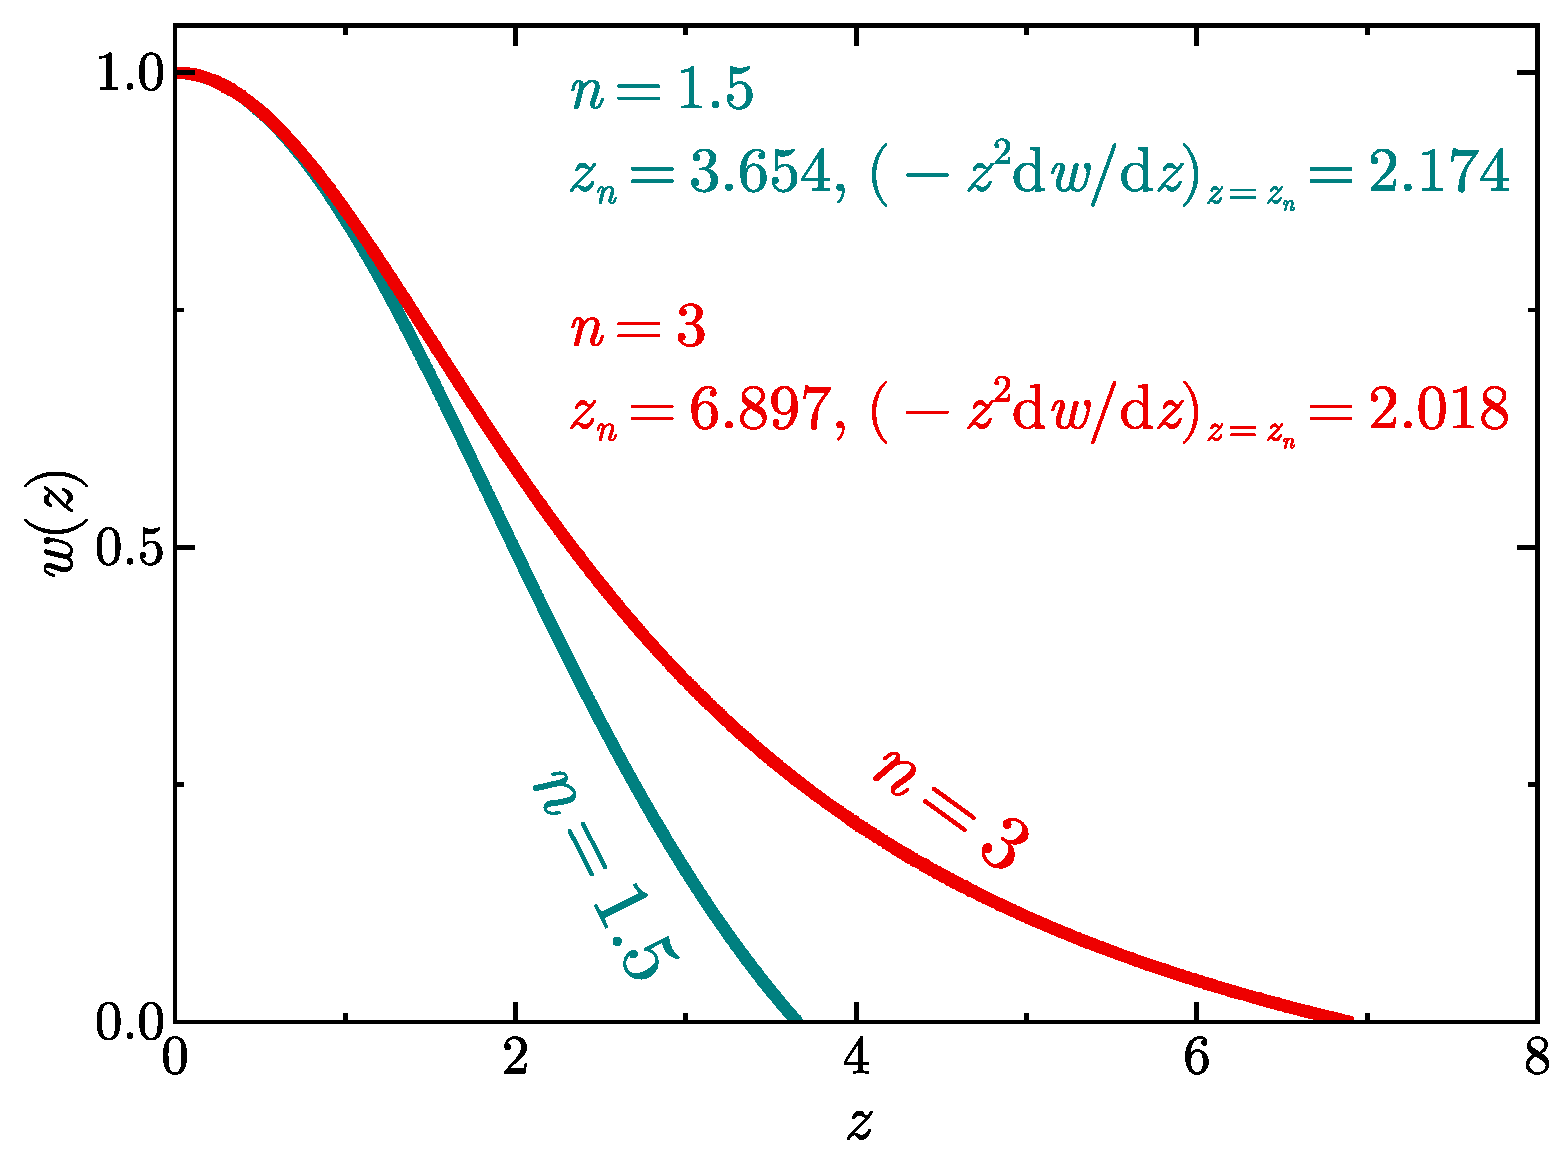
\includegraphics{../assets/4_eos2/polytrope.pdf}
\caption{Solutions to the Lane-Emden equation for $n=3$ and $n=1.5$.}
\end{figure}

As part of the exercises it was also shown that the total mass of a
polytropic model is

\[M=4\pi r_n^3 \rho_\mathrm{c}\left.\left(-z^2\frac{\mathrm{d}w}{\mathrm{d}z}\right)\right|_{z=z_n},\tag{3.4}\]

and that if \(K\) is fixed, we have a mass radius relationship,

\[R\propto M^\beta,\quad \beta=\frac{1-n}{3-n}.\]

let's consider first the non-relativistic case, where \(n=3/2\) which
gives us \(\beta=-1/3\). This means that more massive degenerate stars
are more compact. In turn, this also means that their Fermi momentum is
higher everywhere (as it increases with density), making them more
relativistic. As the mass keeps increasing, we'd expect a star to
approach the extremely relativistic regime, for which \(n=3\). However
this would give us an undefined \(\beta\), meaning the mass radius
relationship is not defined. Why is this the case?

Using the definition of \(r_n\) we can rewrite \((4.3)\) as

\[M=4\pi \left(\frac{(n+1)P_\mathrm{c}}{4\pi G \rho_\mathrm{c}}\right)^{3/2}\rho_\mathrm{c}A_n,\]

where \(A_n\) is just a constant that depends on the polytropic index.
Ignoring all constants (either fixed values from solutions to the
Lane-Emden equation or fundamental constants) we find that

\[M\propto \frac{P_c^{3/2}}{\rho_c^2}=\left(\frac{P_\mathrm{c}^3}{\rho_c^4}\right)^{1/2}.\]

But in the extremely relativistic ,case
\(P_\mathrm{c}\propto \rho_c^{4/3}\), meaning that in this limit \(M\)
has a unique value which is just a function of fundamental constants! If
we properly evaluate all those constants we find that this mass (known
as the Chandrasekhar mass) is:

\[M_\mathrm{Ch}=\frac{5.836}{\mu_e^2}M_\odot,\]

which is equal to \(1.46M_\odot\) for \(\mu_e=2\), characteristing of
white dwarf composition. This is a fundamental limit for the mass of a
star supported by electron pressure degeneracy.

\hypertarget{radiative-energy-transport}{%
\section{Radiative energy transport}\label{radiative-energy-transport}}


\hypertarget{what-is-opacity}{%
\subsection{What is opacity?}\label{what-is-opacity}}

One form in which energy is transported in stellar interiors is through
radiation. However, most of the star is opaque, and photons can only
travel short distances before being scattered or absorbed. The
``opaqueness'' of stellar matter can be described by the opacity
\(\kappa\), which has units of

\[[\kappa]=\mathrm{cm^{2}\,g^{-1}},\]

where brackets denote the units of what is inside.

So what is opacity? Let's start by thinking of a medium with particles
of mass \(m\), which interact with passing radiation. We will consider
each particle acts as a disk of area \(\sigma\) (its cross section), and
that all radiation is absorbed when it hits a particle. We can now
consider a thin slab of material as follows:

\begin{figure}
\centering
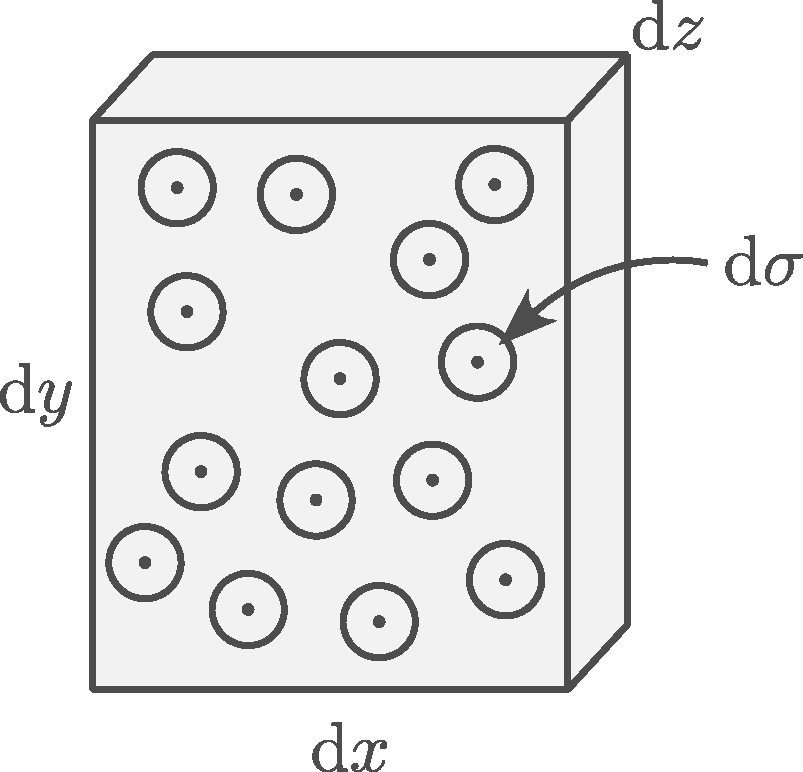
\includegraphics{../assets/5_radiative/opacity.pdf}
\caption{Area covered by particles of cross-area \(\mathrm{d}\sigma\) in
a thin slab.}
\end{figure}

The total number of particles in the slab is

\[dN = \frac{\rho}{m}\mathrm{d}x\mathrm{d}y\mathrm{d}z,\]

which means that the probability of a photon going through the slab and
crashing with a particle is

\[P_\mathrm{coll}=\frac{\sigma \mathrm{d}N}{\mathrm{d}x\mathrm{d}y}=\frac{\sigma \rho}{m}\mathrm{d}z.\]

From here we have the term

\[\left[\frac{\sigma}{m}\right]=\mathrm{cm^2\,g^{-1}},\]

which has the units of opacity. Indeed, opacity can be described as a
cross section per unit mass, and for this specific example we take

\[\kappa\equiv \frac{\sigma}{m}\rightarrow P_\mathrm{coll}=\kappa\rho\mathrm{d}z.\]

Now let's see how flux changes as it goes through the slab:

\begin{figure}
\centering
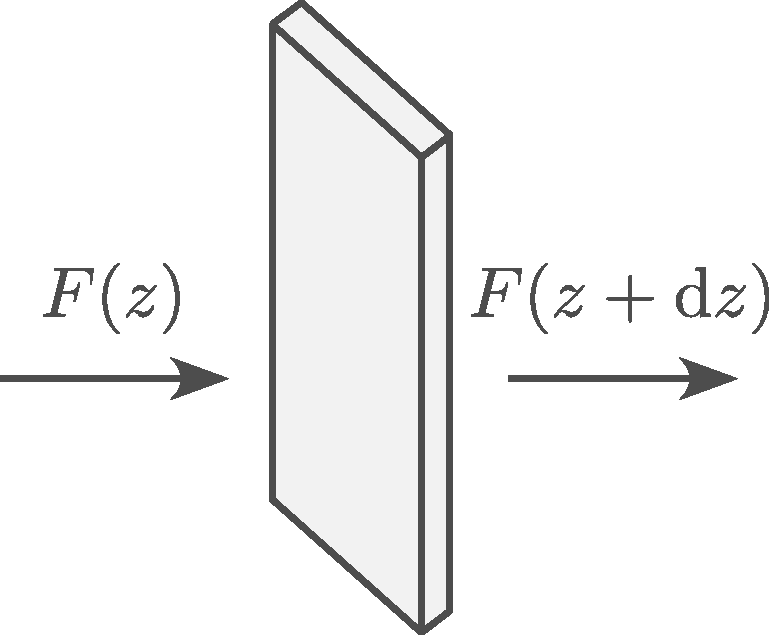
\includegraphics{../assets/5_radiative/flux.pdf}
\caption{Change in flux due to passage through the thin slab.}
\end{figure}

Absent any emission from the slab itself, the difference between the
fluxes at the faces is just

\[F(z)-F(z+\mathrm{d}z)=F(z)P_\mathrm{coll}=F(z)\kappa\rho\mathrm{d}z,\]

and approximating the different in flux with a partial derivative gives
us a differential equation for the flux,

\[\frac{\mathrm{d}F}{\mathrm{d}z} = \kappa\rho F(z).\]

For a constant \(\kappa\rho\), the solution to this differential
equation corresponds to exponential decay,

\[F(z)=F(z_0)e^{-\kappa\rho(z-z_0),}\]

where \(z_0\) is a reference point. From here we have two important
concepts:

\begin{itemize}
\item
  The factor \(\kappa\rho\) in the exponential has units

  \[[\kappa\rho]=\mathrm{cm}^{-1},\]

  so we can define a mean free path for photons as

  \[\displaystyle l_\mathrm{f}=\frac{1}{\kappa\rho}\]

  This corresponds to the typical distance travelled by a photon before
  colliding.

  If we also consider radiation travelling a distance \(d\) through a
  medium, we can define a dimensionless optical depth \(\tau\) as

  \[\tau = \frac{d}{l_\mathrm{f}}=\kappa\rho d.\]

  The optical depth then represents the number of mean free paths
  covered by \(d\). In practice \(\kappa\rho\) varies through a medium,
  so instead one uses

  \[d\tau = \kappa\rho \mathrm{d}z.\]

  For a star, the optical depth normally refers to the value integrated
  from an infinite distance all the way to its surface,

  \[\tau(r) = \int_r^\infty \kappa\rho \mathrm{d}r,\]

  and as we will see later, a usual definition of a stars surface, its
  photosphere, is taken to be at \(\tau=2/3\).
\end{itemize}

\hypertarget{plancks-law}{%
\subsection{Planck's law}\label{plancks-law}}

Let's consider radiation is in local thermodynamical equilibrium with
the gas at a temperature \(T\). Then its energy flux per unit frequency
and solid angle is:

\[B_\nu (\nu,T)=\frac{2h\nu^3}{c^2}\frac{1}{\displaystyle \exp\left(\frac{h\nu}{k_\mathrm{B}T}\right)-1}.\]

What does this imply for the distribution of momenta? Remember that we
defined the distribution \(f(p)\) in terms of the number of particles
per unit volume and unit momentum.

We take an area element \(\mathrm{d}A\), and photons crossing it with a
momentum covering a solid angle \(\mathrm{d}\Omega\) around the
perpendicular direction,

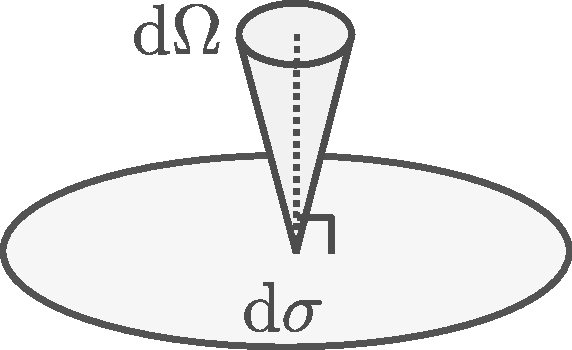
\includegraphics{../assets/5_radiative/intensity.pdf}

In a time \(\mathrm{d}t\), the number of photons crossing
\(\mathrm{d}A\) with directions contained in \(\mathrm{d}\Omega\) is

\[\mathrm{d}N=f(p)c\mathrm{d}t\mathrm{d}A\frac{\mathrm{d}\Omega}{4\pi}\mathrm{d}p,\tag{4.1}\]

where we used the velocity of the photons being the speed of light \(c\)
and took an isotropic \(f(p)\).

Each individual photon carries an energy \(h\nu\), so the energy
corresponding to \(\mathrm{d}N\) is

\[\mathrm{d}E=h\nu \mathrm{d}N.\tag{4.2}\]

Similarly, the momentum of each photon is

\[p=\frac{h\nu}{c}\rightarrow \mathrm{d}p=\frac{h}{c}\mathrm{d}\nu.\tag{4.3}\]

Combining equations \((4.1)\), \((4.2)\) and \((4.3)\) we find that

\[\frac{\mathrm{d}E}{h\nu}=f(p)c\mathrm{d}t\mathrm{d}A\frac{\mathrm{d}\Omega}{4\pi}\frac{h\mathrm{d}\nu}{c}\]
\[\rightarrow \frac{\mathrm{d}E}{\mathrm{d}t\mathrm{d}A\mathrm{d}\Omega\mathrm{d}\nu}=B_\nu = \frac{h^2 \nu}{4\pi}f(p).\]

We can also define the distribution per unit frequency,

\[f(p)\mathrm{d}p=f(\nu)\mathrm{d}\nu \rightarrow \boxed{f(\nu)=\frac{4\pi}{hc\nu}B_\nu.}\tag{4.4}\]

We can use the same expressions as last class to describe the
contribution of radiation to energy density. Expressing the energy
density per unit frequency and unit volume we have

\[U_\nu = f(\nu)h\nu = \frac{4\pi}{c}B_\nu.\]

Similarly, we can describe the flux crossing in one direction of a
surface,

\[F=\int_0^{2\pi}\int_0^{\pi/2}\int_0^\infty \cos\theta\sin\theta B_\nu \mathrm{d}\nu \mathrm{d}\theta \mathrm{d}\phi,\]

which has an analytical solution,

\[F=\sigma T^4,\quad \sigma=\frac{2\pi^5 k_B^4}{15h^3c^2}.\]

The constant \(\sigma\) is known as the Stefan-Boltzmann constant.
Pressure can be found to be equal to

\[P_\mathrm{rad}=\frac{a}{3}T^4,\quad a=\frac{4\sigma}{c},\]

where \(a\) is known as the radiation constant.

Finally, the total energy density (per unit volume) is

\[U=aT^4. \tag{4.5}\]

\hypertarget{basics-of-diffusion}{%
\subsection{Basics of diffusion}\label{basics-of-diffusion}}

If we consider a medium with a density of a particular quantity \(U\)
(per unit volume), moving with a velocity \(v\) and a mean free path
\(l_\mathrm{f}\), then the flux of that property is

\[\vec{F}=-D\nabla U,\quad D=\frac{vl_\mathrm{f}}{3},\tag{4.6}\]

where we have defined the diffusion coefficient \(D\) which has units

\[[D]=\mathrm{cm^{2}\;s^{-1}}.\]

In practice we have multiple velocities and mean free paths, so one
would generally use an average \(\langle vl_\mathrm{f} \rangle\).

The flux described by equation \((4.6)\) needs not just be energy, it
can also describe a flux of particles of different types. Now, we will
not formally derive (4.6), but we will provide a 1-D analogue. Consider
motion only happens in the \(+x\) or \(-x\) direction. We then take an
are \(\mathrm{d}A\) separating two regions of length equal to
\(l_\mathrm{f}\),

\begin{figure}
\centering
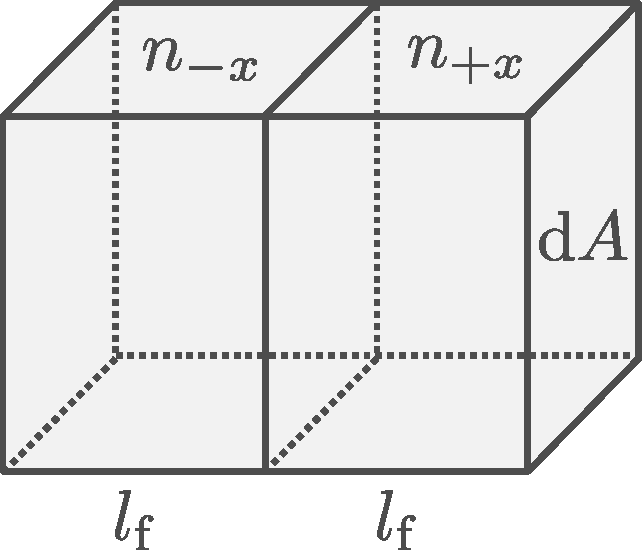
\includegraphics{../assets/5_radiative/diffusion.pdf}
\caption{Neighboring boxes with different particle densities that will
experience diffusive mixing.}
\end{figure}

We approximate the particle density at each side as \(n_{-x}\) and
\(n_{+x}\) with

\[\frac{\mathrm{d}n}{\mathrm{d}x} = \frac{n_{+x}-n_{-x}}{l_\mathrm{f}}.\]

Each box contains a certain amount of particles,

\[\mathrm{d}N_{-x}=n_{-x}\mathrm{d}Al_\mathrm{f},\;\;\mathrm{d}N_{+x}=n_{+x}\mathrm{d}Al_\mathrm{f}.\]

If we take all particles to move with a velocity \(v\) in either the
\(+x\) or \(-x\) direction (with equal probability), then in a time
\(l_\mathrm{f}/v\) half of the particles from each box will cross the
interface, resulting in a flux

\[F_x=\frac{(\mathrm{d}N_{-x}-\mathrm{d}N_{+x})/2}{\mathrm{d}A}\frac{v}{l_\mathrm{f}}\]
\[F_x = -\frac{vl_\mathrm{f}}{2}\frac{\mathrm{d}n}{\mathrm{d}x}.\]

Comparing to equation \((4.6)\), the diffusion coefficient has an
incorrect prefactor, as we have ignored the actual isotropic direction
of the velocities, as well as that particles coming from larger
distances originated from regions of different densities.

\hypertarget{radiative-temperature-gradient}{%
\subsection{Radiative temperature
gradient}\label{radiative-temperature-gradient}}

Now let us consider the flux coming from photon diffusion. For now we
ignore frequency dependency and take all photons to have the same
\(l_\mathrm{f}\),

\[l_\mathrm{f}=\frac{1}{\kappa\rho}.\]

Assuming radial symmetry, equations \((4.5)\) and \((4.6)\) give

\[F_r = \left.-\frac{c}{3\kappa\rho}\frac{\partial U}{\partial r} = -\frac{4acT^3}{3\kappa\rho}\frac{\partial T}{\partial r}\quad\right/4\pi r^2\cdot \tag{4.7}\]
\[L = -\frac{16 \pi r^2 acT^3}{3\kappa\rho}\frac{\partial T}{\partial r}\]
\[\rightarrow \boxed{\frac{\partial T}{\partial r}=-\frac{3\kappa \rho L}{16\pi r^2 a c T^3}}.\tag{4.8}\]

Whenever energy transport happens through radiation, this equation
describes the temperature gradient required. In cases where other
mechanisms transport energy, equation (4.8) describes the radiative
luminosity \(L_\mathrm{rad}\) rather than the total one.

One generally transforms equation (4.8) into a pressure derivative by
using the equation of hydrostatic equilibrium,

\[\frac{\partial P}{\partial r} = -\rho\frac{Gm}{r^2},\]

from which we get

\[\left.\frac{\partial T}{\partial P}=\frac{\partial T}{\partial r}\left(-\frac{r^2}{\rho G m}\right) = \frac{3\kappa L}{16\pi ac G T^3 m}\quad\right/ \frac{P}{T}\cdot\]
\[\boxed{\nabla_\mathrm{rad}\equiv\frac{\partial \ln T}{\partial \ln P}=\frac{3}{16\pi a c G}\frac{\kappa L P}{m T^4}}\tag{4.9}.\]

The quantity \(\nabla_\mathrm{rad}\) will be particularly important in
our discussion of convection in the next class.

In reality we need to consider that opacity is a function of frequency.
In that case we use instead \((4.4)\) and \((4.6)\) to describe the flux
per unit frequency,

\[\vec{F}=-D_\nu \nabla U_\nu,\quad D_\nu = \frac{c}{3\kappa_\nu \rho}.\]

The resulting radial flux per unit frequency can be integrated over
frequency to obtain

\[\nabla_\mathrm{rad}=\frac{3}{16\pi a c G}\frac{\kappa_\mathrm{R} L P}{m T^4},\]

where \(\kappa_\mathrm{R}\) is the Rosseland mean opacity

\[\frac{1}{\kappa_\mathrm{R}}\equiv \frac{\pi}{acT^3}\int_0^\infty\frac{1}{\kappa_\nu}\frac{\partial B_\nu}{\partial T}\mathrm{d}\nu\]

\hypertarget{conduction}{%
\subsection{Conduction}\label{conduction}}

We can also consider conduction in Equation \((4.7)\). The flux can be
taken to be proportional to the temperature gradient, with two
contributions given by conduction coefficients for radiative energy
transport and one for actual particle conduction:

\[\vec{F}=(k_\mathrm{rad}+k_\mathrm{cd})\nabla T,\]

where

\[k_\mathrm{rad}=\frac{4ac}{3}\frac{T^3}{\kappa_\mathrm{rad}\rho}.\]

The conduction coefficient \(\kappa_\mathrm{cd}\) is determined by the
energy density of the particles, their velocity, and their internal
energy density,

\[k_\mathrm{cd}=\frac{lv}{3}\frac{\partial U}{\partial T}.\]

It is common to define a conductive opacity \(\kappa_\mathrm{cd}\) as

\[k_\mathrm{cd}=\frac{4ac}{3}\frac{T^3}{\kappa_\mathrm{cd}\rho},\]

From which we can use the same expression for the temperature gradient
\((4.9)\) but with the opacity replaced with

\[\frac{1}{\kappa}=\frac{1}{\kappa_\mathrm{R}}+\frac{1}{\kappa_\mathrm{cd}}.\]

In this sense the lowest opacity, indicating more transparency,
dominates.

\hypertarget{convection}{%
\section{Convection}\label{convection}}

\hypertarget{schwarzschild-criterion}{%
\subsection{Schwarzschild criterion}\label{schwarzschild-criterion}}

So far we have considered two processes to transport energy, conduction
and radiation. If we were to consider higher and higher luminosities,
while fixing the temperature, density and radius, we would need
increasingly steeper temperature gradients (see equation \((4.8)\)).
But, as we will see now, dynamical instabilities arise if the
temperature gradient becomes too steep.

Let's consider a mass element that is radially displaced upwards a
distance \(\Delta r\).

\begin{figure}
\centering
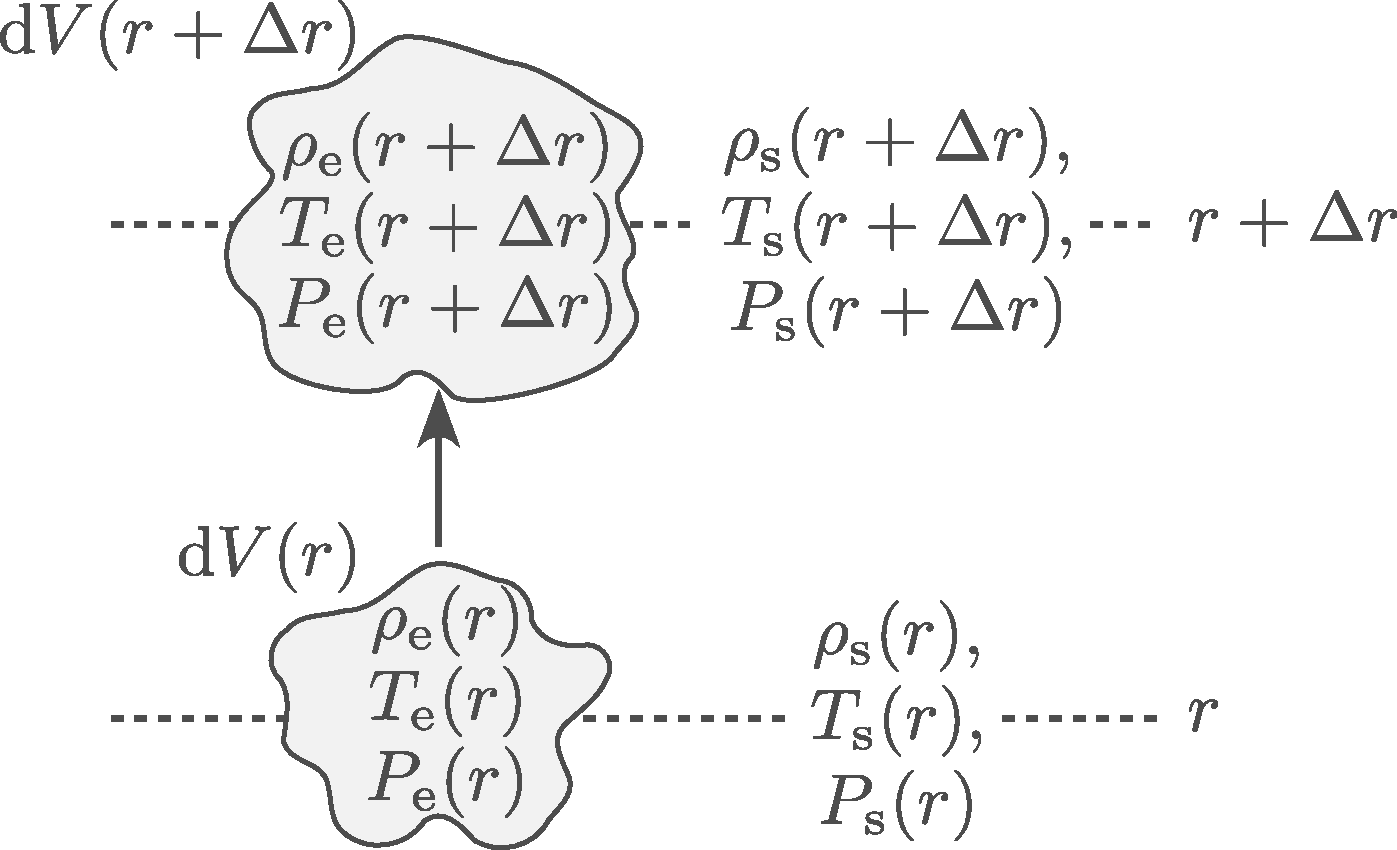
\includegraphics{../assets/6_convection/convection.pdf}
\caption{Change in properties of a convective element compared to its
surroundings.}
\end{figure}

Here we differentiate between properties of the mass element with the
subscript ``e'' and those of its surroundings with a subscript ``s''.
Before the perturbation, we take the properties of the element and its
surroundings to be equal,

\[\rho_\mathrm{e}(r)=\rho_\mathrm{s}(r),\quad T_\mathrm{e}(r)=T_\mathrm{s}(r),\quad P_\mathrm{e}(r)-P_\mathrm{s}(r).\]

We will also consider that the displacement happens slowly, such that
sound waves quickly equalize the pressure of the mass element with its
surroundings as it rises,

\[P_\mathrm{e}(r+\Delta r) = P_\mathrm{s}(r+\Delta r).\]

This requires that the velocity of the moving element is much slower
than the local sound speed.

We can now consider the stability of the displaced element. Let's define
the following quantities:

\[D\rho(r)=\rho_\mathrm{e}(r)-\rho_\mathrm{s}(r), \quad DT(r)=T_\mathrm{e}(r)-T_\mathrm{s}(r).\]

After being displaced a distance \(\Delta r\), the mass element will
experience a radial buoyancy force

\[F_\mathrm{r}=-g D\rho(r+\Delta r)\mathrm{d}V(r),\]

where \(g=Gm(r)/r^2\) is the local gravity. Given this, if for an
upwards displacement (positive \(\Delta r\)) the density of the mass
element becomes smaller than that of its surroundings, there will be a
net outwards force and the system will be unstable. For a small
\(\Delta r\) we can write

\[F_\mathrm{r}=-g\left[\left(\frac{\mathrm{d}\rho}{\mathrm{d}r}\right)_\mathrm{e}-\left(\frac{\mathrm{d}\rho}{\mathrm{d}r}\right)_\mathrm{s}\right]\Delta r \mathrm{d}V(r+\Delta r),\tag{5.1}\]

and requiring \(F_\mathrm{r}<0\) for \(\Delta r>0\) we obtain a
stability criterion:

\[\left(\frac{\mathrm{d}\rho}{\mathrm{d}r}\right)_\mathrm{e}-\left(\frac{\mathrm{d}\rho}{\mathrm{d}r}\right)_\mathrm{s}>0.\tag{5.2}\]

The same result is obtained if we take a perturbation with
\(\Delta r=0.\)

In practice, we use a different version of the instability criterion
that depends on the temperature gradient. Let's consider the
relationship between changes in density, temperature and pressure
(ignoring composition variation for simplicity):

\[\frac{\mathrm{d}\rho}{\rho}=\alpha\frac{\mathrm{d}P}{P}-\delta\frac{\mathrm{d}T}{T},\]

where

\[\alpha=\left(\frac{\partial \ln\rho}{\partial \ln P}\right)_T,\quad \delta=-\left(\frac{\partial \ln \rho}{\partial \ln T}\right)_P.\]

Using this the left hand side of equation \((5.2)\) can be rewritten as

%\[\left(\frac{\mathrm{d}\rho}{\mathrm{d}r}\right)_\mathrm{e}-\left(\frac{\mathrm{d}\rho}{\mathrm{d}r}\right)_\mathrm{s}=\cancel{\frac{\alpha\rho}{P}\left(\frac{\mathrm{d}P}{\mathrm{d}r}\right)_\mathrm{e}} - \frac{\delta\rho}{T}\left(\frac{\mathrm{d}T}{\mathrm{d}r}\right)_\mathrm{e} - \cancel{\frac{\alpha\rho}{P}\left(\frac{\mathrm{d}P}{\mathrm{d}r}\right)_\mathrm{s}} + \frac{\delta\rho}{T}\left(\frac{\mathrm{d}T}{\mathrm{d}r}\right)_\mathrm{s},\tag{5.3}\]
\[\left(\frac{\mathrm{d}\rho}{\mathrm{d}r}\right)_\mathrm{e}-\left(\frac{\mathrm{d}\rho}{\mathrm{d}r}\right)_\mathrm{s}=\cancel{\frac{\alpha\rho}{P}\left(\frac{\mathrm{d}P}{\mathrm{d}r}\right)_\mathrm{e}} - \frac{\delta\rho}{T}\left(\frac{\mathrm{d}T}{\mathrm{d}r}\right)_\mathrm{e}\]
\[\qquad\qquad\qquad\qquad\qquad\qquad- \cancel{\frac{\alpha\rho}{P}\left(\frac{\mathrm{d}P}{\mathrm{d}r}\right)_\mathrm{s}} + \frac{\delta\rho}{T}\left(\frac{\mathrm{d}T}{\mathrm{d}r}\right)_\mathrm{s},\tag{5.3}\]

where the pressure derivatives cancel from our assumption of a slowly
rising element.

Consider now the pressure scale height, defined as

\[H_P\equiv -P\left(\frac{\mathrm{d}P}{\mathrm{d}r}\right)^{-1}.\]

The pressure scale height serves as a measure of the length scale over
which the stellar interior changes. In the case of hydrostatic
equilibrium we have

\[H_P = \frac{P}{\rho g}.\]

Multiplying \((5.3)\) by \(H_P\) can be used to turn the radial
derivatives into pressure derivatives,

\[H_P\left[\left(\frac{\mathrm{d}\rho}{\mathrm{d}r}\right)_\mathrm{e}-\left(\frac{\mathrm{d}\rho}{\mathrm{d}r}\right)_\mathrm{s}\right]=\frac{\delta \rho P}{T}\left[\left(\frac{\mathrm{d}T}{\mathrm{d}P}\right)_\mathrm{e}-\left(\frac{\mathrm{d}T}{\mathrm{d}P}\right)_\mathrm{s}\right]\]
\[=\delta\rho\left[\left(\frac{\mathrm{d}\ln T}{\mathrm{d}\ln P}\right)_\mathrm{e} - \left(\frac{\mathrm{d}\ln T}{\mathrm{d}\ln P}\right)_\mathrm{s}\right].\tag{5.4}\]

The temperature gradient with respect to pressure in the surroundings of
the mass element is the definition of \(\nabla\),

\[\nabla\equiv\left(\frac{\mathrm{d}\ln T}{\mathrm{d}\ln P}\right)_\mathrm{s}.\]

In contrast to \(\nabla_\mathrm{rad}\), this is the actual temperature
gradient of the star, while \(\nabla_\mathrm{rad}\) represents the
gradient required for all the luminosity to be transported by radiation
(or also, conduction). If we consider the mass element is displaced
adiabatically,

\[\left(\frac{\mathrm{d}\ln T}{\mathrm{d}\ln P}\right)_\mathrm{e}=\nabla_\mathrm{ad},\]

and equation \((5.4)\) is

\[\left(\frac{\mathrm{d}\rho}{\mathrm{d}r}\right)_\mathrm{e}-\left(\frac{\mathrm{d}\rho}{\mathrm{d}r}\right)_\mathrm{s} = \frac{\delta\rho}{H_P}(\nabla_\mathrm{ad}-\nabla),\tag{5.5}\]

and the stability condition of equation \((5.1)\) reduces to

\[\boxed{\nabla_\mathrm{ad}>\nabla.}\]

This is known as the Schwarzschild criterion.

\hypertarget{brunt-vuxe4isuxe4luxe4-frequency}{%
\subsection{Brunt-Väisälä
frequency}\label{brunt-vuxe4isuxe4luxe4-frequency}}

Before discussing what happens if the fluid is unstable to convection,
let's see how a perturbation evolves with time. Combining \((5.1)\) and
\((5.5)\) we get the equation of motion

\[\mathrm{d}m\frac{\mathrm{d}^2\Delta r}{\mathrm{d}t^2}=-\frac{g\delta\rho}{H_P}(\nabla_\mathrm{ad}-\nabla)\Delta r \mathrm{d}V(r+\Delta r)\tag{5.6}.\]

For the volume \(\mathrm{d}V\) we have

\[\mathrm{d}V(r+\Delta r)=\frac{\mathrm{d}m}{\rho(r+\Delta r)}=\frac{\mathrm{d}m}{\displaystyle\rho(r)+\Delta r\left(\frac{\mathrm{d}\rho}{\mathrm{d}r}\right)_\mathrm{e}}\]
\[\qquad\qquad\qquad\qquad\qquad\simeq \frac{\mathrm{d}m}{\rho(r)}\left[1-\frac{\Delta r}{\rho}\left(\frac{\mathrm{d}\rho}{\mathrm{d}r}\right)_\mathrm{e}\right],\]

so to first order in \(\Delta r\) equation \((5.6)\) is

\[\frac{\mathrm{d}^2\Delta r}{\mathrm{d}t^2}=-\frac{g\delta}{H_P}(\nabla_\mathrm{ad}-\nabla)\Delta r.\tag{5.7}\]

The solution to this equation consists of oscillatory behavior or
exponential growth, depending on the sign of
\(\nabla_\mathrm{ad}-\nabla\),

\[\Delta r = (\Delta r)_0 \exp(i\omega_\mathrm{BV}(t-t_0)),\]

where \(\omega_\mathrm{BV}\) is the Brunt-Väisälä frequency

\[\omega_\mathrm{BV}^2 = \frac{g\delta}{H_P}\left(\nabla_\mathrm{ad}-\nabla\right).\]

In regions of a star where \(\nabla_\mathrm{ad}>\nabla\) (meaning,
convectively stable) \(\omega_\mathrm{BV}\) defines a natural frequency
of oscillations within the star.

Note that in our discussion on stability we have not considered the
effect of possible composition gradients, which can develop naturally
inside a star as a consequence of nuclear burning. How that affects the
instability criterion (and thus, the Brunt-Väisälä frequency) is studied
in the exercises of this session.

\hypertarget{mixing-length-theory}{%
\subsection{Mixing length theory}\label{mixing-length-theory}}

So, what happens if the fluid is unstable to convection? Then we will
have energy transported through advection. If we consider a mass element
travels a distance \(l\) before dissolving and equalizing its
temperature with its environment, then it will release an amount of heat

\[Q = \mathrm{d}m c_P DT(r+l).\tag{5.8}\]

As convection requires \(\nabla_\mathrm{ad}<\nabla\), and pressure
decreases outwards, we expect \(DT(r+l)\) to be positive for positive
\(l\) and negative otherwise. This implies that convection indeed
transports energy outwards.

But how much energy flux do we expect? In principle this is a very
complex 3D hydrodynamics problem, which is unfeasible to compute
together with the long evolutionary timescales of stars. Instead, the
most common approach is a 1D approximation known as mixing length theory
(MLT). Here we will show an example of MLT which does not account for
radiative losses of energy from a mass element as it is displaced.

As small perturbations induce instability, let's assume that a
convective region is entirely composed of blobs of materials that are
unstable and move up or down. We consider a slab of material of area
\(\mathrm{d}A\), and consider the mass elements crossing it in a time
\(\mathrm{d}t\),

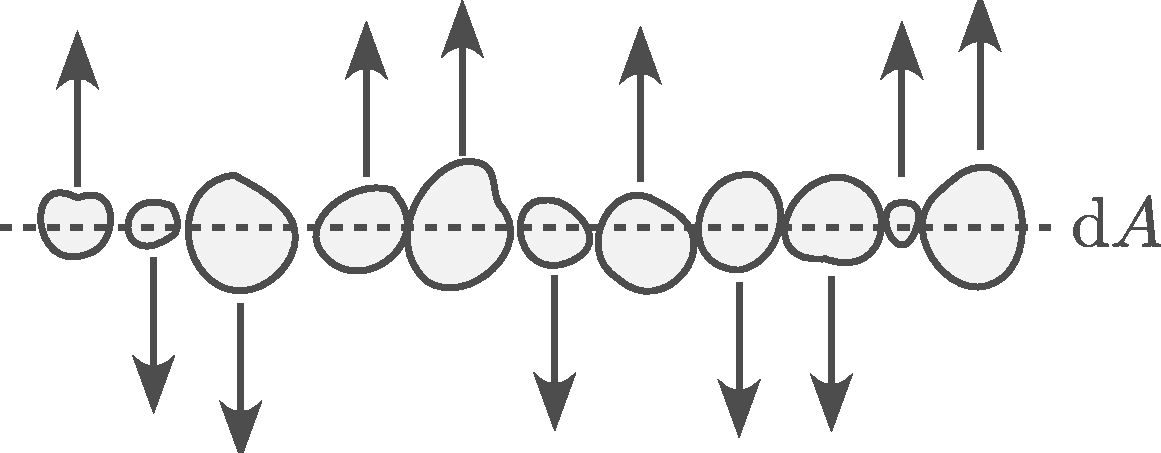
\includegraphics{../assets/6_convection/blobs.pdf}

These elements have different velocities, sizes and temperature
contrasts \(DT\). We simplify things by taking all elements to have a
characteristic absolute velocity \(|v|\) and absolute temperature
contrast \(|DT|\) (positive for rising elements, negative otherwise).
The amount of mass crossing \(\mathrm{d}A\) upwards in time
\(\mathrm{d}t\) is

\[\mathrm{d}M_+=\frac{1}{2}\rho|v|\mathrm{d}A\mathrm{d}t,\]

and similarly the mass crossing downwards is

\[\mathrm{d}M_-=\frac{1}{2}\rho|v|\mathrm{d}A\mathrm{d}t=\mathrm{d}M_+.\]

The total energy flux can be estimated by considering the heat excess
given by equation \((5.8)\). As \(v\) and \(DT\) are positive for
elements moving radially upwards, they produce a net outwards radial
energy flow. The same applies to downwards moving elements, which have a
negative \(v\) and negative \(DT\).

Dropping the absolute values to simplify notation and taking \(v\) and
\(DT\) as positive, the flux coming from upwards and downwards moving
mass elements totals

\[F=\rho v c_P DT.\tag{5.9}\]

We will take as a characteristic length traveled by the mass element at
the moment it crosses \(\mathrm{d}A\) to be half of their total travel
distance \(l_\mathrm{MLT}\). The distance \(l_\mathrm{MLT}\) is a-priori
unknown, and it is the reason for the name ``mixing-length-theory''. For
a displacement \(l_\mathrm{MLT}/2\) we have for \(DT\)

\[DT=\frac{l_\mathrm{MLT}}{2}\left.\left[\left(\frac{\mathrm{d}T}{\mathrm{d}r}\right)_\mathrm{e}-\left(\frac{\mathrm{d}T}{\mathrm{d}r}\right)_\mathrm{s}\right]\quad\right/\cdot H_P\]

\[H_P DT = -\frac{Pl_\mathrm{MLT}}{2}\left[\left(\frac{\mathrm{d}T}{\mathrm{d}P}\right)_\mathrm{e}-\left(\frac{\mathrm{d}T}{\mathrm{d}P}\right)_\mathrm{s}\right]\]

\[DT=-\frac{l_\mathrm{MLT}T}{2H_P}\left[\left(\frac{\mathrm{d}\ln T}{\mathrm{d}\ln P}\right)_\mathrm{e}-\left(\frac{\mathrm{d}\ln T}{\mathrm{d}\ln P}\right)_\mathrm{s}\right]\]

\[DT = -\frac{l_\mathrm{MLT}T}{2H_P}(\nabla-\nabla_\mathrm{ad}),\tag{5.10}\]

which as we have mentioned is positive for a positive \(l_\mathrm{MLT}\)
in a convective region, as the Schwarzschild criterion requires
\(\nabla>\nabla_\mathrm{ad}\). The quantity
\((\nabla-\nabla_\mathrm{ad})\) is known as the superadiabaticity.

We then need to compute the characteristic velocity \(v\). Using
equation \((5.7)\) we can estimate the work done on the fluid element
after it has traveled a distance \(l_\mathrm{MLT}/2\),

\[W=\int_0^{l_\mathrm{MLT}/2}\mathrm{d}m\frac{g\delta}{H_P}(\nabla-\nabla_\mathrm{ad})\Delta r\mathrm{d}(\Delta r)\]
\[= \mathrm{d}m\frac{g\delta}{H_P}(\nabla-\nabla_\mathrm{ad})\frac{l_\mathrm{MLT}^2}{4}.\]

Not all of this work is translated into kinetic energy, as the gas also
does work by expanding as it rises, pushing matter around. It is in
details such as those that different forms of MLT arise. To recover a
standard form of the convective flux, we will assume a quarter of \(W\)
goes into kinetic energy,

\[\frac{1}{2}\mathrm{d}m v^2 = \frac{W}{4}\]

\[\rightarrow v=\left(\frac{g\delta}{H_P}\right)^{1/2}(\nabla-\nabla_\mathrm{ad})^{1/2}\frac{l_\mathrm{MLT}}{2\sqrt{2}}.\]

From this expression for the convective velocity we get the convective
flux using equations \((5.9)\) and \((5.10)\),

\[\boxed{F_\mathrm{conv}=\rho c_P T \sqrt{g\delta} \frac{l_\mathrm{MLT}^2}{4\sqrt{2}}H_P^{-3/2}(\nabla-\nabla_\mathrm{ad})^{3/2}.}\]

From this equation we see that the larger the superadiabaticity, the
larger the convective flux. In many situations we find that the
prefactor to \((\nabla-\nabla_\mathrm{ad})^{3/2}\) in
\(F_\mathrm{conv}\) is so large that in practice the star only needs a
small superadiabaticity \((\nabla-\nabla_\mathrm{ad})\ll 1\) to
transport its energy outwards. In that case a coarse approximation of a
structure equation for a convective region is to have

\[\nabla = \nabla_\mathrm{ad}.\]

This is however not generally applicable, as radiative losses can make
convection inefficient particularly in the outermost layers of a star.

\hypertarget{nucleosynthesis}{%
\section{Nucleosynthesis}\label{nucleosynthesis}}

For reference, this section is based on chapter 6 of the lectures on
stellar evolution by Onno Pols, available at
\url{https://www.astro.ru.nl/~onnop/education/stev_utrecht_notes/}.

\hypertarget{basic-definitions}{%
\subsection{Basic definitions}\label{basic-definitions}}

We have by now discussed how energy is transported through a star, but
have not considered in much detail how it is generated. A natural source
of energy is contraction, where a star sinks into its own potential well
to provide its surface luminosity. However, through most of a stars
lifetime the main source of energy comes from nuclear fusion reactions.

Typical notations for reactions are

\[X+a\rightarrow Y+b\quad \text{or} \quad X(a,b)Y.\]

In here it could be read that \(X\) produces \(Y\) by interacting with
\(a\), releasing \(b\) as a side product. But in practice \(X\) and
\(a\) have equivalent roles in the reaction. Any such reaction must
satisfy two basic conservation laws

\begin{itemize}
\tightlist
\item
  Conservation of baryon number
\item
  Conservation of charge
\end{itemize}

The first conservation law can be taken as that the sum of protons and
neutrons must remain constant.

The reason why nuclear reactions allow for a release of energy is that
due to nuclear forces the rest mass energy of an atomic nucleus is
different from that of its constituent neutrons and protons if they were
free particles. Considering the actual mass \(m_i\) of a nucleus with
atomic number \(A_i\), its binding energy is defined as

\[E_{\mathrm{b},i}=[(A_i-Z_i)m_n + Z_i m_p - m_i]c^2.\]

If we consider the most common isotopes for each element, one can see
how the energy per baryon varies with mass number (image source:
\href{https://commons.wikimedia.org/wiki/File:Binding_energy_curve_-_common_isotopes.pdf}{Wikimedia
Commons}),

\begin{figure}
\centering
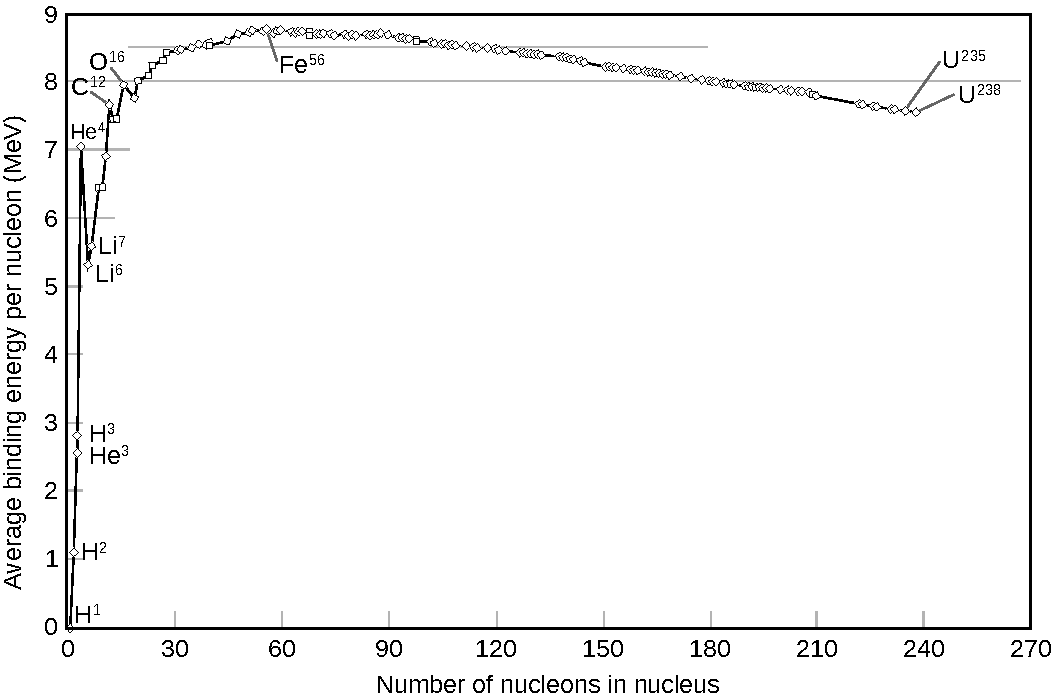
\includegraphics{../assets/7_nucleo1/binding.pdf}
\caption{Binding energy of most common isotopes.}
\end{figure}

We see that the most bound nucleus is \(^{56}\mathrm{Fe}\). This means
that by fusing lighter atoms we can release energy (exothermic
reactions), but once we burn everything into iron any additional fusion
process requires energy (endothermic reaction). The formation of an iron
core then represents a critical evolutionary stage, as we will see
later.

The energy released by a reaction rate can be determined by taking the
mass difference between the initial and final states,

\[Q=(m_X+m_a-M_Y-m_b)c^2.\tag{6.1}\]

In some cases some of this energy is, however, lost. This is the case
when neutrinos are produced, which can have large energies and can
travel pretty much unimpeded from the stellar core to its surface.

In order to compute (6.1), one can make use of atomic masses. However,
note that these are for neutral atoms, so they include electron masses!

\hypertarget{cross-sections-rates}{%
\subsection{Cross sections \& rates}\label{cross-sections-rates}}

Just as wit the interaction of light and matter, nuclear reactions are
characterized by cross sections. If we consider fixed particles \(X\)
against which a flux (particles per unit area) of particles \(a\) is
shot, then the cross section for the reaction is defined as

\[\sigma = \frac{\begin{matrix}\text{\# of reactions $X(a,b)Y$ per unit time} \\ \text{per \# of $X$ particles}\end{matrix}}{\text{flux of $a$ in frame of $X$}}.\]

If the relative velocity between particles \(X\) and \(a\) is \(v\),
then the flux of \(a\) in the frame of \(X\) is simply \(n_av\) (where
\(n_a\) are the number of \(a\) particles per unit volume). For
arbitrary particles \(i\) and \(j\) we can then write the number of
reactions per unit time and unit volume as

\[\tilde{r}_{ij}=n_i n_j v \sigma.\]

There is a small caveat for the case of equal particles reacting
together. In that case, if we have \(N\) particles the total number of
pairings without double counting is

\[\frac{1}{2}N(N-1)\sim \frac{N^2}{2}\quad(\text{for $N\gg 1$}),\]

so the general form of the reaction rate is

\[\tilde{r}_{i,j}=\frac{1}{1+\delta_{ij}}n_in_jv\sigma\]

where \(\delta_{ij}\) is the Kronecker delta.

In practice, inside a star we have a distribution of relative velocities
between particles, and the cross section is different at different
velocities. The rate then comes from integrating over all relative
velocities,

\[r_{ij}=\frac{1}{1+\delta_{ij}}n_in_j\underbrace{\int_0^\infty f(v)\sigma(v)v\mathrm{d}v}_{\equiv \langle\sigma v\rangle}.\tag{6.2}\]

Here \(f(v)\) has a different meaning to previous sections where we used
\(f\) to denote the number density of particles per unit something. Here
\(f\) is the distribution of relative velocities, which is a normalized
property:

\[\int_o^\infty f(v)\mathrm{d}v=1.\]

Luckily for us, if both types of particles have a Maxwellian
distribution then \(f(v)\) also has a Maxwellian form,

\[f(v)=4\pi v^2\left(\frac{m}{2\pi k_\mathrm{B}}\right)^{3/2}\exp\left(-\frac{mv^2}{2k_\mathrm{B}T}\right),\quad m=\frac{m_im_j}{m_i+m_j}.\]

Changing integration variable in \((6.2)\) from velocity to energy
(non-relavistic, so \(E=mv^2/2\)) one has

\[\langle\sigma v\rangle=\left(\frac{8}{\pi m}\right)^{1/2}(k_\mathrm{B}T)^{-3/2}\int_0^\infty \sigma(E)E\exp\left(-\frac{E}{k_\mathrm{B}T}\right)\mathrm{d}E.\tag{6.3}\]

The whole dependence of the nuclear reaction rate on temperature is then
condensed in this factor.

For the purpose of solving the equations of stellar structure and
evolution we need to know the specific nuclear energy generation rate
\(\varepsilon_\mathrm{nuc}\). For a reaction rate with a \(Q\)-value
\(Q_{ij}\) and rate per unit volume \(r_{ij}\), one has

\[\varepsilon_\mathrm{nuc}=\frac{Q_{ij}r_{ij}}{\rho},\]

where in practice one adds up over all possible reactions.

\hypertarget{tunneling-the-gamow-peak}{%
\subsection{Tunneling \& the Gamow
peak}\label{tunneling-the-gamow-peak}}

For two nuclei with atomic numbers \(Z_1\) and \(Z_2\), their
interaction is described by a potential that is dominated by nuclear
forces at very small separations and by the Coulomb potential farther
away.

\begin{figure}
\centering
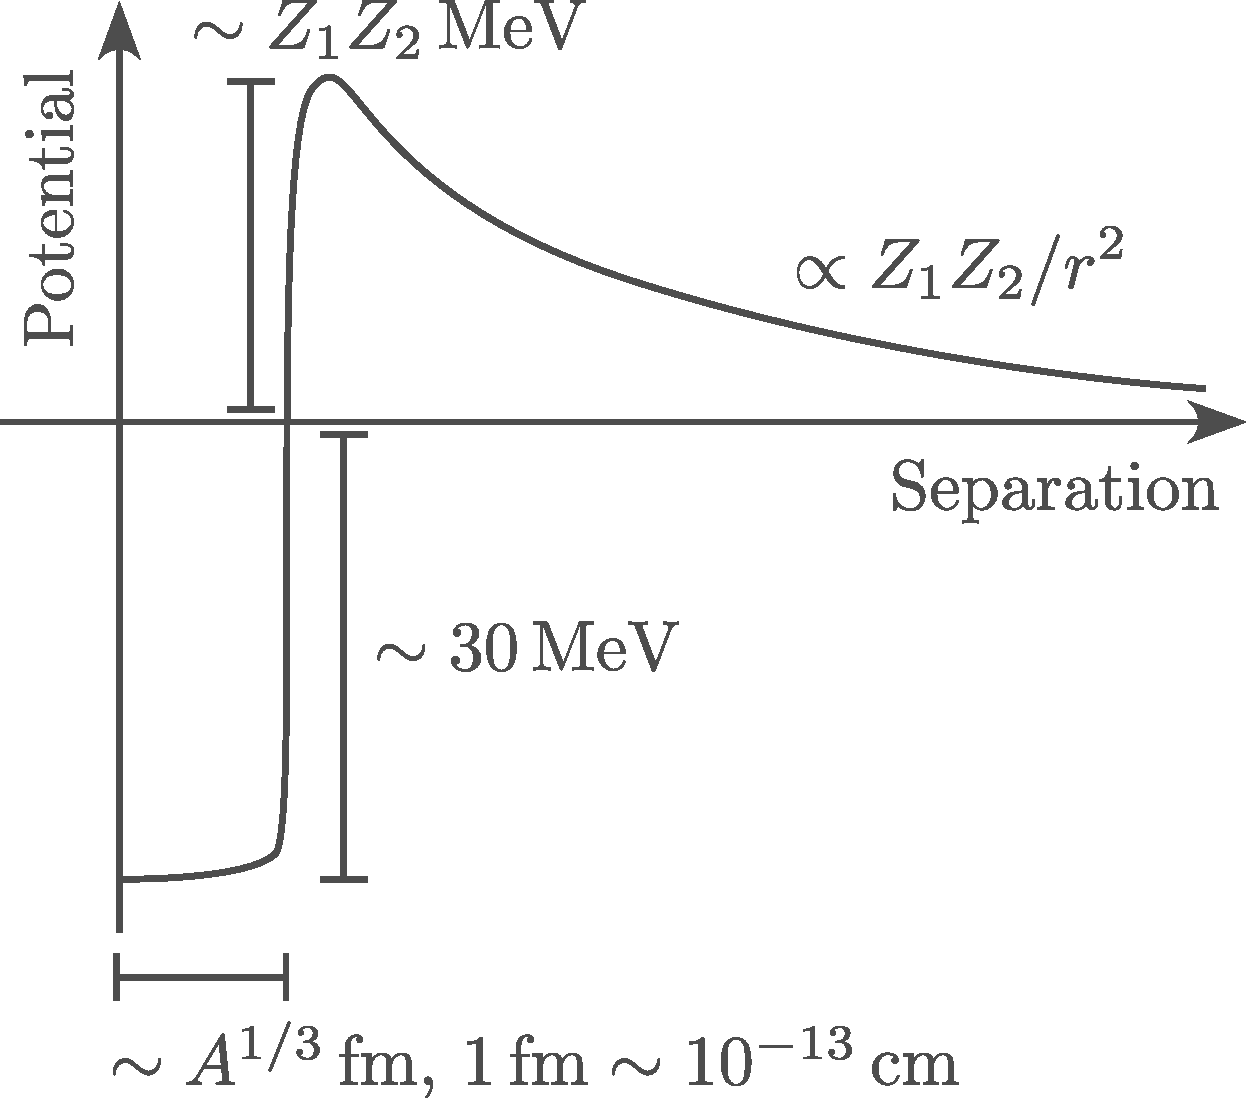
\includegraphics{../assets/7_nucleo1/potential.pdf}
\caption{Illustration of the nuclear potential.}
\end{figure}

If we consider the core of the Sun, which has a temperature of order
\(10^7\) Kelvin, the typical particle energy is
\(\sim k_\mathrm{B}T\sim \mathrm{keV}\). In a classical picture, we need
\(\mathrm{MeV}\) energies to go above the Coulomb potential and produce
a nuclear reaction. One could think it is still possible considering the
high energy tail of a Maxwell-Boltzmann distribution, but the
probability of having even a single particle with enough energy is
vanishingly small.

So, we need quantum mechanics to explain how nuclear reactions can
happen at all in the solar core. A particle with momentum \(p\) has a
corresponding wavelength that characterizes it, called the \emph{de
Broglie} wavelength:

\[\lambda = \frac{\hbar}{p},\text{ normally $\gg A^{1/3}\,\mathrm{fm}$}.\]

This allows for quantum tunneling to produce nuclear reactions even if
the energy is too low to overcome the Coulomb barrier. Formally
computing the cross section while accounting for this shows that the
cross section is

\[\sigma(E)\sim \pi \lambda^2\underbrace{\exp(-b E^{-1/2})}_\text{Tunneling factor},\]

where

\[b=2\pi \frac{Z_i Z_j e^2}{\hbar}\left(\frac{m}{2}\right)^{1/2}=31.29 Z_iZ_j A^{1/2}\,[\mathrm{keV}^{1/2}].\]

Here \(A\equiv A_iA_j/(A_i+A_j)\) is the reduced mass number. The factor
\(b\) ensures that different burning stages are well separated in
temperature as tunneling of particles with a smaller \(Z\) is
significantly favored.

Since \(p^2/(2m)=E\), one usually writes

\[\sigma(E)=S(E)\frac{\exp\left(-bE^{-1/2}\right)}{E},\tag{6.4}\]

where \(S(E)\), called the S-factor, quantifies variations over the
regular expected behavior. Often \(S(E)\) varies very slowly compared to
\(\sigma(E)\), allowing, for example, to extrapolate cross sections
determined in the laboratory to energies relevant to stellar interiors.
The S-factor can, however, have strong variations due to particular
resonances at specific interaction energies.

If we apply equation \((6.4)\) to equation \((6.3)\), we find that

\[\langle\sigma v\rangle = f(T,m)\int_0^\infty S(E)\exp\left(-bE^{-1/2}-\frac{E}{k_\mathrm{B}T}\right)\mathrm{d}E.\tag{6.5}\]

Excluding the S-factor, the exponential term in the integral is such
that it peaks at a narrow range of energies, as depicted below.

\begin{figure}
\centering
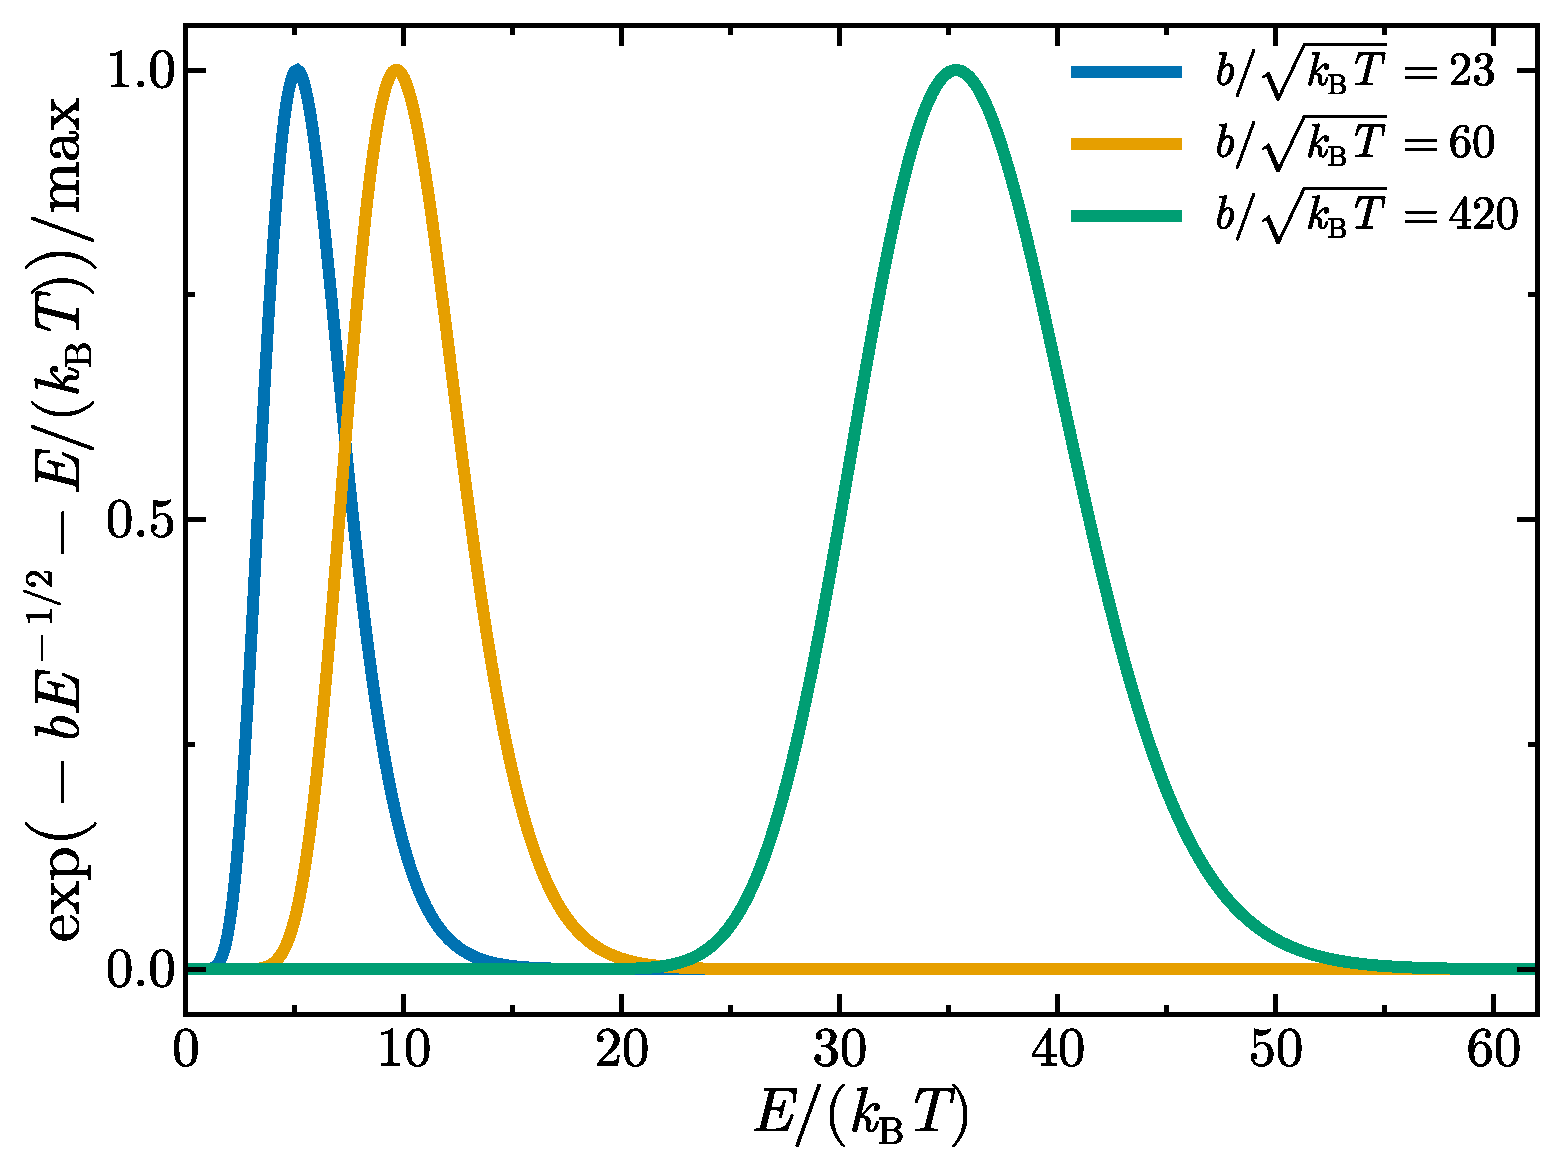
\includegraphics{../assets/7_nucleo1/gamow.pdf}
\caption{Gamow peak.}
\end{figure}

This figure shows the value of the exponential term in equation
\((6.5)\) (normalized by its maximum) for different values of the ratio
\(b/\sqrt{k_\mathrm{B}T}\). These values are chosen to be representative
of hydrogen burning at a temperature of \(10^7\,\mathrm{K}\), helium
burning at \(10^8\,\mathrm{K}\) and carbon burning at
\(5\times 10^{8}\,\mathrm{K}\). This function is commonly referred to as
the Gamow peak, and can to first order be approximated with a Gaussian
function. In that case, if one assumes \(S(E)\) does not vary
significantly within the range of energies relevant to the Gamow peak,
it can be taken off the integral in equation (6.5), which can then be
evaluated analytically (see exercises for this session).

\hypertarget{nuclear-burning-stages}{%
\subsection{Nuclear burning stages}\label{nuclear-burning-stages}}

\hypertarget{main-sequence}{%
\subsubsection{Main sequence}\label{main-sequence}}

As under specific conditions tunneling is favored for the particles with
lower \(Z\), the first (and longer-lasting) phase of nuclear burning of
a star is that of core-hydrogen burning, were hydrogen is fused into
helium. This stage is known as the main-sequence, and the onset of
core-hydrogen burning is known as the zero-age main sequence. As a
hydrogen atom is composed of a single baryon, while helium consists of
4, we need a series of reactions to build it up. The identification of
the specific set of reactions that are dominant in stellar evolution led
to the discovery of two different burning processes. The first one is
the PP-chain, which in its simpler form (called the PP-I chain), is what
one might think as the most natural way to fuse four hydrogen atoms into
helium. This is depicted in the figure below.

\begin{figure}
\centering
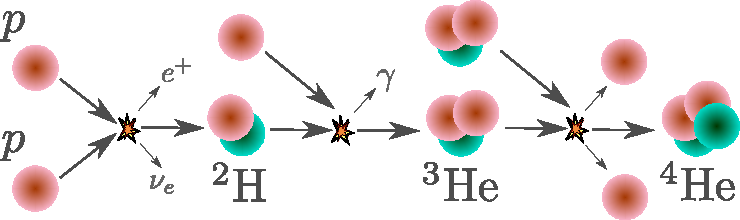
\includegraphics{../assets/7_nucleo1/PPI.pdf}
\caption{PP-I chain.}
\end{figure}

However, it is found that for stars with masses above
\(\sim 1.5M_\odot\), a different and much less intuitive process is
dominant, known as the CNO cycle. The CNO cycle uses carbon, nitrogen
and oxygen as catalysts, where through a series of hydrogen fusion
processes with the CNO elements and beta decays helium can be produced
without modifying the total number of CNO atoms. The figure below
illustrates the CNO-I (left loop) and CNO-II (right loop) cycles.

\begin{figure}
\centering
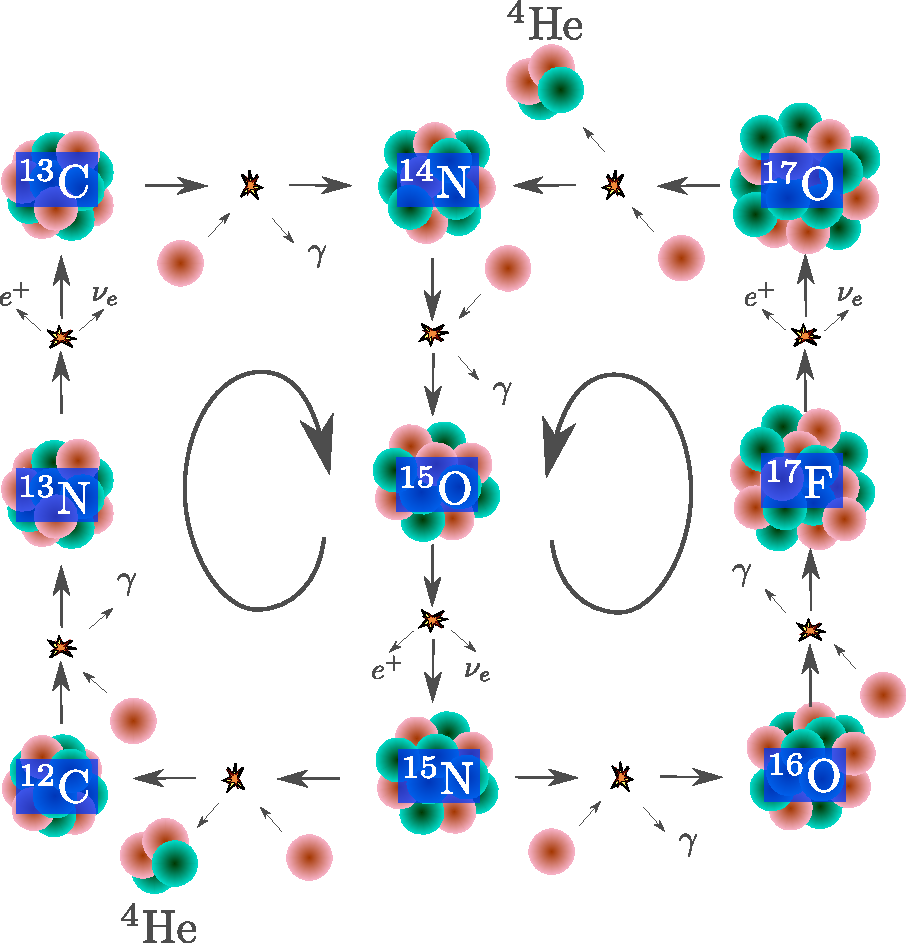
\includegraphics{../assets/7_nucleo1/CNO.pdf}
\caption{CNO-I and CNO\_II burning processes.}
\end{figure}

Based on the Gamow peak, nuclear energy production rates can be
approximated around a specific temperature in terms of a power-law index
\(\nu\) (see exercises for this session):

\[\varepsilon_\mathrm{nuc}=\varepsilon_0 \rho T^\nu.\]

For main-sequence stars it is found that for PP burning one has
\(\nu\simeq4\), while for CNO burning \(\nu\simeq 18\). The scaling of
nuclear reactions is incredibly sensitive to temperature!

\hypertarget{beyond-the-main-sequence}{%
\subsubsection{Beyond the main
sequence}\label{beyond-the-main-sequence}}

After a star depletes its central hydrogen, depending on conditions
we'll discuss next chapter, it will start burning heavier elements. In
particular, lower mass stars can undergo only a subset of the reactions
discussed below. The outcome of the main-sequence is to produce a helium
core, at which point the core will lose its energy source and start
contracting. This leads to shell burning of hydrogen and potentially the
ignition of helium in its core. This process is repeated after core
helium exhaustion, resulting on shell helium burning and potentially the
ignition of nuclear fusion involving heavier nuclei at its core. Below
we indicate the main processes operating after the main-sequence, and
the characteristic central temperatures \(T_\mathrm{c}\) at which they
operate.

\begin{itemize}
\item
  Helium burning, \(T_\mathrm{c}>10^8\,\mathrm{K}\).

  The main reaction during this stage is known as the triple-\(\alpha\)
  reaction, where three helium atoms (\(\alpha\) particles) are fused
  into carbon. The first stage consists on the production of an unstable
  beryllium atom,

  \[^4\mathrm{He}+^4\mathrm{He}\leftrightarrow ^8\mathrm{Be}.\]

  The half-life of \(^8\mathrm{Be}\) is very short, on the order of
  \(10^{-16}\) seconds, so the beryllium nucleus needs to rapidly fuse
  with another alpha particle before decaying. The most likely process
  involves the production of an excited state of carbon, denoted as
  \(^{12}\mathrm{C}^*\), which rapidly decays into the ground state of
  the carbon nucleus,

  \[^8\mathrm{Be}+^4\mathrm{He}\leftrightarrow ^{12}\mathrm{C}^*\rightarrow ^{12}\mathrm{C}+\gamma.\]

  The full triple-\(\alpha\) process can then be summarized as

  \[3\,{^4}\mathrm{He}\rightarrow ^{12}\mathrm{C}+\gamma.\]

  Towards the end of helium burning, as the core temperature increases
  during this phase, \(\alpha\) captures on the carbon nucleus also
  become important,

  \[^{12}\mathrm{C}+^{4}\mathrm{He}\rightarrow ^{16}\mathrm{O}+\gamma,\]

  such that the end result of core-helium burning is the production of a
  carbon-oxygen core. The
  \(^{12}\mathrm{C}(\alpha,\gamma)^{16}\mathrm{O}\) reaction has
  important uncertainties at the conditions relevant in stellar
  interiors, which affects the resulting ratio of carbon and oxygen at
  the end of helium burning.
\item
  Carbon burning, \(T_\mathrm{c}>5\times 10^8\,\mathrm{K}.\)

  Carbon burning proceeds through the fusion of two carbon nuclei into
  an excited state of magnesium, which then decays into either neon or
  sodium:

  \[^{12}\mathrm{C}+^{12}\mathrm{C}\rightarrow ^{24}\mathrm{Mg}^*
  \begin{array}{l}
  \rightarrow ^{20}\mathrm{Ne}+\alpha\\
  \rightarrow ^{23}\mathrm{Na}+\mathrm{p}
  \end{array}\]

  owing to the large temperature, the released \(\alpha\) particle or
  proton in these reactions can rapidly fuse with the surrounding atoms.
  The net result of core carbon burning is then a core formed of
  \(^{16}\mathrm{O}\), \(^{20}\mathrm{Ne}\) and \(^{25,26}\mathrm{Mg}\).
\item
  Neon burning, \(T_\mathrm{c}>1.5\times 10^9\,\mathrm{K}.\)

  Although one would naturally expect oxygen burning to follow after
  carbon burning, what happens instead is an endothermic reaction
  involving neon. The \(^{20}\mathrm{Ne}\) atom is not very stable, and
  before oxygen ignites there are sufficient high energy photons to
  destroy the neon atom,

  \[^{20}\mathrm{Ne}+\gamma\rightarrow ^{16}\mathrm{O}+\alpha.\]

  This process where high energy photons destroy nuclei is called
  photodisintegration. As for the case of carbon burning, the resulting
  \(\alpha\) particle can rapidly fuse, in particular leading to the
  production of magnesium,

  \[^{20}\mathrm{Ne}+\gamma \rightarrow ^{24}\mathrm{Mg}+\gamma.\]
\item
  Oxygen burning, \(T_\mathrm{c}>2\times 10^9\,\mathrm{K}.\)

  Similar to carbon burning, oxygen burning proceeds through the fusion
  of two oxygen atoms into an excited nuclear state (in this case of
  sulfur), which then can decay into two different atoms.

  \[^{16}\mathrm{O}+^{16}\mathrm{O}\rightarrow ^{32}\mathrm{S}^*
  \begin{array}{l}
  \rightarrow ^{28}\mathrm{Si}+\alpha\\
  \rightarrow ^{31}\mathrm{P}+\mathrm{p}
  \end{array}\]

  The resulting proton and alpha particle can quickly fuse with
  surrounding nuclei, leading to a core composition mostly composed of
  \(^{28}\mathrm{Si}\) and \(^{32}\mathrm{S}\).
\item
  Silicon burning, \(T_\mathrm{c}>3\times 10^9\,\mathrm{K}.\)

  By the point oxygen is depleted, the core is mostly composed of
  silicon, but at this stage the Coulomb barrier of the silicon atom
  turns out to be prohibitively high, preventing the fusion of two
  silicon atoms. Instead, high energy photons are actually capable of
  producing a series of photodisintegration processes, effectively
  undoing the cycle of nuclear reactions up to this point:

  \[^{28}\mathrm{Si}(\gamma,\alpha)^{24}\mathrm{Mg}(\gamma,\alpha)^{20}\mathrm{Ne}(\gamma,\alpha)^{16}\mathrm{O}(\gamma,\alpha)^{12}\mathrm{C}(\gamma,\alpha)^{24}2\alpha.\]

  Simultaneously, the released \(\alpha\) particles can fuse with
  surrounding nuclei, leading to the production of heavier elements:

  \[^{28}\mathrm{Si}(\alpha,\gamma)^{32}\mathrm{S}(\alpha,\gamma)^{36}\mathrm{Ar}(\alpha,\gamma)^{40}\mathrm{Ca}(\alpha,\gamma)^{44}\mathrm{Ti}(\alpha,\gamma)^{32}\mathrm{S}\dots^{56}\mathrm{Ni}.\]

  The resulting nickel atom can then decay into \(^{56}\mathrm{Fe}\), at
  which point we have reached the nucleus with the highest binding
  energy. This is a critical stage of evolution, as no exothermic
  reactions are possible beyond that stage. The end result is that the
  iron core will grow until a point where it experiences a dynamical
  core-collapse phase, potentially producing a compact object (neutron
  star or black hole) with an associated supernova event.
\end{itemize}

The end result of all these burning processes is that the star ends up
with an onion-layer like structure, with the deeper regions of the star
corresponding to the later nuclear burning phases.

\hypertarget{main-sequence-homology}{%
\section{Main sequence homology}\label{main-sequence-homology}}

For reference, this section is based on chapter 7 of the lectures on
stellar evolution by Onno Pols, available at
\url{https://www.astro.ru.nl/~onnop/education/stev_utrecht_notes/}.

\hypertarget{homology}{%
\subsection{Homology}\label{homology}}

So far we have derived a series of equations of stellar structure and
evolution. Here we will consider stable stellar models, where we take
time derivatives to be negligible to the other terms. We have

\[\frac{\mathrm{d}r}{\mathrm{d}m}=\frac{1}{4\pi r^2\rho},\quad\text{Continuity equation}\]
\[\frac{\mathrm{d}P}{\mathrm{d}m}=-\frac{Gm}{4\pi r^4},\quad\text{Hydrostatic equilibrium (HSE)}\]
\[\frac{\mathrm{d}L}{\mathrm{d}m}=\varepsilon_\mathrm{nuc},\quad\text{Energy equation}\]
\[\frac{\mathrm{d}T}{\mathrm{d}m}=-\frac{Gm}{4\pi r^4}\frac{T}{P}\nabla,\quad
\nabla=\begin{cases}
\nabla_\mathrm{rad},\;\nabla_\mathrm{rad}<\nabla_\mathrm{ad} \\
\nabla_\mathrm{ad},\;\nabla_\mathrm{rad}>\nabla_\mathrm{ad} &
\end{cases}\]

The last equation, which comes from the mode of energy transport, is
often called the temperature equation. Beware that
\(\nabla=\nabla_\mathrm{ad}\) is a significant simplification, as for
convection to transport any energy at all we need
\(\nabla>\nabla_\mathrm{ad}\), as we discussed when we derived a form of
mixing-length theory. Since we are considering static models, we drop
the partial derivative signs.

The equations above pose a significant problem, as even if we make
simplistic assumptions about opacities and nuclear reaction rates they
are highly non-linear and are not amicable to find analytical solutions.
So instead, we will take a different approach. Consider we have a star
of mass \(M_1\) for which we have a solution to the structure equations,
meaning we know \(r_1(m)\), \(P_1(m)\), \(T_1(m)\) and \(L_1(m)\). We
will then consider a star of mass \(M_2\), together with a corresponding
solution \(r_2(m)\), \(P_2(m)\), \(T_1(2)\) and \(L_2(m)\). To relate
both models we will write the equations of stellar structure in terms of
a relative mass coordinate

\[x=\frac{m_1}{M_1}=\frac{m_2}{M_2}.\]

For each star, quantities at the same \(x\) then mean that we consider
them at the same relative mass coordinate. Now, we will assume that both
models are such that their radii follow

\[\frac{r_1(x)}{r_2(x)}=\frac{R_1}{R_2}.\tag{7.1}\]

Such two models are called homologous, which means layers of both models
at the same mass coordinate are related by a fixed expansion or
contraction factor.

Under the assumption of homology we can study how different solutions
behave with changing mass and radius, without actually knowing any
solution precisely. We do this by considering what \((7.1)\) implies for
the solution to the equations of stellar structure for the second star.
We apply this logic to each of the equations of stellar structure in the
following subsections.

\hypertarget{continuity-equation-1}{%
\subsubsection{Continuity equation}\label{continuity-equation-1}}

Let's start by considering the continuity equation for star 1:

\[\frac{\mathrm{d}r_1}{\mathrm{d}m_1}=\frac{1}{4\pi r_1^2 \rho_1}.\]

We can replace the derivative with one with respect to \(x\),

\[\frac{\mathrm{d}r_1}{\mathrm{d}m_1}=\frac{\mathrm{d}r_1}{\mathrm{d}x}\frac{\mathrm{d}x}{\mathrm{d}m_1}=\frac{1}{M_1}\frac{\mathrm{d} r_1}{\mathrm{d}x},\]

such that

\[\frac{\mathrm{d}r_1}{\mathrm{d}x}=\frac{M_1}{4\pi r_1^2 \rho_1}.\tag{7.2}\]

Homology requires that \(r_1=r_2(R_1/R_2)\), so replacing on the left
hand side we get

\[\left(\frac{R_1}{R_2}\right)\frac{\mathrm{d}r_2}{\mathrm{d}x}=\frac{M_1}{4\pi r_1^2\rho_1},\]

but \((7.2)\) must also hold by swapping indexes \(1\rightarrow 2\), so

\[\left(\frac{R_1}{R_2}\right)\frac{M_2}{4\pi r_2^2 \rho_2}=\frac{M_1}{4\pi r_1^2 \rho_1}.\]

Finally, applying \((7.1)\) again we find that

\[\boxed{\frac{\rho_1(x)}{\rho_2(x)}=\frac{M_1}{M_2}\left(\frac{R_1}{R_2}\right)^{-3}},\tag{7.3}\]

\hypertarget{equation-of-hydrostatic-equilibrium}{%
\subsubsection{Equation of Hydrostatic
Equilibrium}\label{equation-of-hydrostatic-equilibrium}}

Now we will work with the equation of hydrostatic equilibrium (HSE).
Similar to before, we find that

\[\frac{\mathrm{d}P}{\mathrm{d}x}=-\frac{Gm_1M_1}{4\pi r_1^4},\]
\[=-\frac{Gm_2M_2}{4\pi r_2^4}\left(\frac{m_1}{m_2}\right)\left(\frac{M_1}{M_2}\right)\left(\frac{r_2^4}{r_1^4}\right),\]
\[=\frac{\mathrm{d}P_2}{\mathrm{d}x}\left(\frac{M_1}{M_2}\right)^2\left(\frac{R_1}{R_2}\right)^{-4}.\]

We can integrate this for an arbitrary \(x\) up to the surface
(\(x=1\)), where ignoring surface pressure we obtain

\[\boxed{\frac{P_1(x)}{\mathrm{P_2(x)}}=\left(\frac{M_1}{M_2}\right)^2\left(\frac{R_1}{R_2}\right)^{-4}}\tag{7.4}\]

\hypertarget{equation-of-state}{%
\subsubsection{Equation of state}\label{equation-of-state}}

By using the equation of state we can also connect pressure, density
temperature and composition. Lets consider an ideal gas equation of
state, without radiation pressure and a fixed mean molecular weight
\(\mu\),

\[P=\frac{\rho}{\mu m_\mathrm{u}}k_\mathrm{B}T.\]

We can consider this EOS for both stars with potentially different
\(\mu_1\) and \(\mu_2\), in which case we get

\[\frac{P_1}{P_2}=\frac{\rho_1}{\rho_2}\left(\frac{\mu_1}{\mu_2}\right)^{-1}\frac{T_1}{T_2}.\]

Using \((7.3)\) and \((7.4)\) we find

\[\left(\frac{M_1}{M_2}\right)^2\left(\frac{R_1}{R_2}\right)^{-4}=\frac{M_1}{M_2}\left(\frac{R_1}{R_2}\right)^{-3}\left(\frac{\mu_1}{\mu_2}\right)^{-1}\frac{T_1}{T_2}\]
\[\rightarrow \boxed{\frac{T_1(x)}{T_2(x)}=\frac{\mu_1}{\mu_2}\frac{M_1}{M_2}\left(\frac{R_1}{R_2}\right)^{-1}}\tag{7.5}\]

\hypertarget{radiative-energy-transport-1}{%
\subsubsection{Radiative energy
transport}\label{radiative-energy-transport-1}}

Next, we will consider radiative energy transport. We have that

\[\frac{\mathrm{d}(T_1^4)}{\mathrm{d}x}=-\frac{3\kappa_1 l_1 M_1}{16\pi^2 a c r_1^4},\tag{7.6}\]

where we use \(l=L(M)\) to reserve \(L\) for the surface luminosity. We
assume a general power-law form for the opacity,

\[\kappa = \kappa_0 \rho^a T^b. \tag{7.7}\]

For bound-free and free-free opacity, the Kramer's law indicates \(a=1\)
and \(b=3.5\) in particular. As one of the exercises of today's session
it is shown that \((7.5)\), \((7.6)\) and \((7.7)\) imply that

\[\left(\frac{T_1(x)}{T_2(x)}\right)^4=\frac{l_1(x)}{l_2(x)}\frac{M_1}{M_2}\frac{\kappa_1}{\kappa_2}\left(\frac{R_1}{R_2}\right)^{-4}.\]

Further applying \((7.5)\) provides the homology relationship for
luminosity:

\[\boxed{\frac{l_1(x)}{l_2(x)}=\left(\frac{\mu_1}{\mu_2}\right)^4\left(\frac{M_1}{M_2}\right)^3\left(\frac{\kappa_1}{\kappa_2}\right)^{-1}}.\tag{7.8}\]

From this we see that the surface luminosity of homologous models scales
steeply with mass,

\[L\propto \kappa^{-1}\mu^{4}M^3.\]

Note that this is independent of the energy source powering the star!

\hypertarget{main-sequence-homology-1}{%
\subsection{Main sequence homology}\label{main-sequence-homology-1}}

The relationships derived so far allow us to determine how the different
properties of a homogeneous star scale with mass and radius. These
relationships can be used to describe a star that is out of thermal
equilibrium, where its energy source comes from sinking in its own
potential well. Placing an extra homology constraint can the allow us to
determine a mass-radius relationship. We can do this by applying the
equation of thermal equilibrium,

\[\frac{\mathrm{d}l}{\mathrm{d}m}=\varepsilon_\mathrm{nuc}.\]

It is by including this that we have information on the nuclear burning
process and can thus discuss the main sequence (meaning, the
core-hydrogen burning phase). From the exercises of the previous class
we saw that one can approximate a reaction rate using a power law in
temperature, such that

\[\varepsilon_\mathrm{nuc}=\varepsilon_0 \rho T^\nu.\]

With this the equation of thermal equilibrium reads

\[\frac{\mathrm{d}l_1}{\mathrm{d}x}=\varepsilon_0 M_1 \rho_1 T_1^\nu\]
\[=\frac{\mathrm{d}l_2}{\mathrm{d}x}\frac{M_1}{M_2}\frac{\rho_1}{\rho_2}\left(\frac{T_1}{T_2}\right)^\nu.\]

All terms in parenthesis are not functions of \(x\) given \((7.3)\) and
\((7.5)\) so we can integrate from the core to an arbitrary \(x\) to
find (where we take \(l(0)=0\)),

\[\frac{l_1(x)}{l_2(x)}=\frac{M_1}{M_2}\frac{\rho_1}{\rho_2}\left(\frac{T_1}{T_2}\right)^\nu.\]

But we already have homology relationships for \(l(x)\) (eq. \((7.8)\)),
\(\rho(x)\) (eq. \((7.3)\)) and \(T(x)\) (eq. \((7.5)\)). If we make use
of these we get

\[\left(\frac{\mu_1}{\mu_2}\right)^4\left(\frac{M_1}{M_2}\right)^3\left(\frac{\kappa_1}{\kappa_2}\right)^{-1}=\qquad\qquad\qquad\qquad\qquad\qquad\qquad\]
\[\frac{M_1}{M_2}\cdot \frac{M_1}{M_2}\left(\frac{R_1}{R_2}\right)^{-3}\cdot \left(\frac{\mu_1}{\mu_2}\right)^\nu\left(\frac{M_1}{M_2}\right)^\nu\left(\frac{R_1}{R_2}\right)^{-\nu},\]

From which we get a direct relationship between the mass and the radius,

\[\frac{R_1}{R_2}=\left(\frac{\mu_1}{\mu_2}\right)^{(\nu-4)/(\nu-3)}\left(\frac{M_1}{M_2}\right)^{(\nu-1)/(\nu+3)}\left(\frac{\kappa_1}{\kappa_2}\right)^{1/(\nu+3)}.\]

For the conditions at which stars undergo PP and CNO burning in their
cores one has that \(\nu\simeq 4\) and \(\nu\simeq 18\) respectively.
So, ignoring the dependence in opacity, we see that the radius of the
star at the zero-age main sequence (start of hydrogen burning with
homogeneous composition) is expected to increase with mass. Although
this might appear obvious, it is not. In particular this is the opposite
to what we found for degenerate stars, which we can approximate through
polytropic models that have a decreasing radius with mass.

\hypertarget{main-sequence-and-beyond}{%
\section{Main sequence and beyond}\label{main-sequence-and-beyond}}

\hypertarget{eddington-grey-boundary-conditions}{%
\subsection{Eddington grey boundary
conditions}\label{eddington-grey-boundary-conditions}}

So far we have made the simplification \(P(M)=0\), as this makes
analytical solutions easier. But in practice a star has a fuzzy
atmosphere, where at some point radiation decouples from matter and most
photons stream freely outwards. As collisions become less frequent, with
larger mean free paths, matter as well deviates from a state of local
thermodynamical equilibrium. Normally when we compute a stellar model we
restrict the simulation domain to its photosphere, for which we havee an
effective temperature \(T_\mathrm{eff}\). This temperature can be
defined as

\[L(R_\mathrm{p})=4\pi R_\mathrm{p}^2\sigma T_\mathrm{eff}^4,\]

and the photosphere radius \(R_\mathrm{p}\) is the location where

\[T(R_\mathrm{p})=T_\mathrm{eff}.\]

said differently, it is the point that satisfies

\[T(R_\mathrm{p})=\left(\frac{L(R_\mathrm{p})}{4\pi R_\mathrm{p}^2\sigma}\right)^{1/4}.\]

Formally treating a stellar atmosphere is quite an involved process, so
we usually make use of an approximation devised by Arthur Eddington, the
Eddington grey atmosphere. Grey refers to ignoring opacity variations
throughout the atmosphere. We start with the result we derived when
studying radiative energy transport, which says that in a radiative
layer the temperature gradient is giveen by

\[\frac{\partial T}{\partial r}=-\frac{3\kappa \rho L}{16acT^3\pi r^2},\quad P_\mathrm{r}=\frac{a}{3}T^4.\tag{8.1}\]

Since we have

\[\frac{\partial P_\mathrm{r}}{\partial r}=\frac{4}{3}aT^3\frac{\partial T}{\partial r},\]

we can write \((8.1)\) as

\[\frac{\partial P_\mathrm{r}}{\partial r}=-\frac{-\kappa\rho}{c}\frac{L}{4\pi r^2}.\tag{8.2}\]

As we move away from the photosphere, the radiation field \(I_\nu\)
(flux per unit frequency, time and solid angle in a specific direction)
deviates from isotropy and instead points preferentially outwards. At
this point \((8.1)\) does not hold as \(I_\nu\neq B_\nu\) and we
assumed a Planck distribution for radiation to derive it. However, the
Eddington approximation still uses \((8.2)\) with the radiation
pressure being given by

\[P_\mathrm{r}=\int_0^{2\pi}\int_0^\pi\int_0^\infty\frac{I_\nu(\theta,\phi)}{c}\cos^2\theta\sin\theta\mathrm{d}\nu\mathrm{d}\theta\mathrm{d}\phi.\]

The above epression can be derived using similar arguments to our
derivation of pressure from an isotropic distribution of momenta. Taking
\(\theta\) to be the polar angle with respect to the radial direction
and assuming radial symmetry we have
\(I_\nu(\theta,\phi)=I_\nu(\theta)\). Moreover, we have

\[\int_0^\infty I_\nu(\theta) \mathrm{d}\nu=I(\theta),\]

such that

\[P_\mathrm{r}=\frac{2\pi}{c}\int_0^\pi I(\theta)\cos^2(\theta)\sin(\theta)\mathrm{d}\theta,\]
\[=\frac{2\pi}{c}\int_{-1}^1I(\mu)\mu^2\mathrm{d}\mu,\;\mu\equiv\cos\theta.\]

Similarly, the flux is given by

\[F=2\pi\int_{-1}^1 I(\mu)\mu \mathrm{d}\mu,\]

which applies throughout the entire star, meaning that we always need at
least a small amount of anisotropy to transport energy through
radiation. In practice in the deep stellar interior tiny variations from
\(B_\nu\) are sufficient for this.

Now let us assume we have a thin photosphere where

\[\frac{L(r)}{4\pi r^2}=F(r)\simeq \mathrm{constant},\]

and let us use optical depth as a variable,

\[\mathrm{d}\tau=-\kappa\rho\mathrm{d}r,\quad \tau=0\quad \mathrm{at}\quad r=\infty,\]

which allows us to rewrite \((8.2)\) as

\[\frac{\partial P_\mathrm{r}}{\partial\tau}=\frac{F}{c}\rightarrow P_\mathrm{r}=\frac{F}{c}\tau+P_\mathrm{\tau=0}.\tag{8.3}\]

In the Eddington approximation we assume that across the atmosphere we
also have

\[P_\mathrm{r}=\frac{1}{3}aT^4,\]

and we also take the intensity to be constant in outgoing directions,

\[I(\mu,\tau=0)=\begin{cases}I_0 & 0\leq \mu \leq 1 \\ 0 & -1 \leq \mu < 0.\end{cases}\]

Computing the pressure and flux associated to this we get

\[P_r(\tau=0)=\frac{2\pi}{c}\int_0^1I_0\mu^2\mathrm{d}\mu=\frac{2\pi}{3c}I_0,\]
\[F(\tau=0)=2\pi\int_0^1I_0\mu\mathrm{d}\mu=\pi I_0,\]

such that

\[P_\mathrm{\tau=0}=\frac{2F(\tau=0)}{3c}.\]

Replacing in \((8.3)\) together with the assumption of constant flux
through the thin atmosphere we get

\[\frac{1}{3}aT^4=\frac{F}{c}\tau +\frac{2F}{3c}=\frac{2F}{3c}\left(\frac{3}{2}\tau + 1\right)\]

and finally, sincee \(F=\sigma T_\mathrm{eff}^4, we have that\)

\[T^4=\frac{T_\mathrm{eff}^4}{2}\left(\frac{3}{2}\tau+1\right).\]

This gives us that the optical depth of the photosphere, where
\(T=T_\mathrm{eff}\), is at \(\tau_\mathrm{p}=2/3\). In a stellar model
we can set the outer boundary to be at \(\tau=2/3\) and use as a
boundary condition on temperature that

\[T(\tau=2/3)=\left(\frac{L(\tau=2/3)}{4\pi [r(\tau=2/3)]^2\sigma}\right)^{1/4}.\]

This is not enough though, as we need an additional outer boundary
condition. For this purpose we can build a boundary condition using the
equation of hydrostatic equilibrium,

\[\frac{\partial P}{\partial r}=-g\rho,\quad g\equiv \frac{Gm(r)}{r^2}.\]

Changing variables to \(\tau\) we get

\[\frac{\partial P}{\partial \tau}=\frac{g}{\kappa}.\]

By using the thin atmosphere approximation, with
\(g\simeq g_\mathrm{s}\equiv GM/R^2\) taken as a constant, together with
the grey atmosphere approximation (\(\kappa=\mathrm{constant}\)) we find
that

\[P(\tau=2/3)=\frac{2g_\mathrm{s}}{3\kappa(\tau=2/3)}+P(\tau=0).\]

The pressure at \(P(\tau=0)\) is given by \(P_\mathrm{r}(\tau=0)\), but
in many cases it can be neglected. It is important though for very
luminous stars near the Eddington limit.

\hypertarget{the-main-sequence-in-the-hertzsprung-russel-diagram}{%
\subsection{The main sequence in the Hertzsprung-Russel
diagram}\label{the-main-sequence-in-the-hertzsprung-russel-diagram}}

Now that we have a way to connect luminosity and radius to effective
temperature, we can use our homology relationships to discuss the shape
of the main sequence. We start from the mass radius relationship that we
derived for both PP and CNO burning,

\[R\propto M^{0.43}\;\mathrm{(PP)},\quad R\propto M^{0.81}\;\mathrm{(CNO)}.\]

We also derived a mass luminosity relationship,

\(L\propto M^3,\)

although the opacity dependence can have a significant impact on the
exponent that we ignore now. We can relate \(R\) and \(L\) to the
effective temperature,

\[T_\mathrm{eff}^4 \propto \frac{L}{R^2},\]

which combined with the mass-radius and mass-luminosity relationships
above give us the scaling of the effective temperature with mass for
zero-age main sequence stars.

\[T_\mathrm{eff}\propto M^{0.54}\;\mathrm{(PP)},\quad T_\mathrm{eff}\propto M^{0.35}\;\mathrm{(CNO)}.\]

This reproduces qualitatively the properties of the main sequence where
more massive and luminous stars have a higher effective temperature.
Additionally, luminosities cover several orders of magnitude for stars
of different masses while variations in effective temperature are much
more limited.

We can also make use of our surface boundary conditions to determine the
properties of another prominent feature in the HR diagram, the Hayashi
line. This is the locus populated by fully convective stars for which a
specific opacity source (\(\mathrm{H}^{-}\)) is critical. The physics of
the Hayashi line are much more involved though, and it is left as a
reading assignment (Chapter 24 of the Kippenhahn textbook).

\hypertarget{basic-main-sequence-structure}{%
\subsection{Basic main sequence
structure}\label{basic-main-sequence-structure}}

A simple thing we can check is how stars transition from PP to CNO
burning being dominant as we consider higher masses. In particular we
have from zero-age main-sequence homology that the central temperature
scales with mass as

\[T_\mathrm{c}\propto M^{-0.29}\;\mathrm{(PP)},\;M^{-1.4}\;\mathrm{(CNO)}.\]

If we consider the ratio between the energy generation rates from PP and
CNO, we find that

\[\frac{\varepsilon_{\mathrm{PP,c}}}{\varepsilon_{\mathrm{CNO,c}}}=\frac{\varepsilon_{\mathrm{0,PP}\rho_\mathrm{c}}T_\mathrm{c}^{\nu,\mathrm{PP}}}{\varepsilon_{\mathrm{0,CNO}}\rho_\mathrm{c}T_\mathrm{c}^{\nu,\mathrm{CNO}}}\propto T_\mathrm{c}^{\nu,\mathrm{PP}- \nu,\mathrm{CNO}},\tag{8.4}\]

where we distinguish between the power exponents for PP
(\(\nu,\mathrm{PP}\simeq 4\)) and CNO burning
(\(\nu,\mathrm{CNO}\simeq 18\)). Let us assume that at a certain mass
burning is completely dominated by the PP chain, such that the
relationship \(T_\mathrm{c}\propto M^{-0.29}\) for PP burning holds and
\((8.4)\) gives

\[\frac{\varepsilon_{\mathrm{PP,c}}}{\varepsilon_{\mathrm{CNO,c}}}\propto M^{0.57(\nu,\mathrm{PP}- \nu,\mathrm{CNO})}.\]

The exponent is significantly smaller than zero, meaning that there is a
narrow range in masses where there is a switch between PP burning being
absolutely dominant and CNO burning being the one dominating energy
generation. This also serves to justify our use of either PP burning or
CNO burning for the scaling of \(\varepsilon_\mathrm{nuc}\).

The shift from PP to CNO drives an important change on how energy is
transported in stellar interiors. Stars with masses similar to the Sun
have radiative cores and convective envelopes, while the inverse is the
case for more massive stars, the shift being around \(1.5M_\odot\).
Stars below \(\sim0.5M_\odot\) are completely convective during the main
sequence.

\begin{figure}
\centering
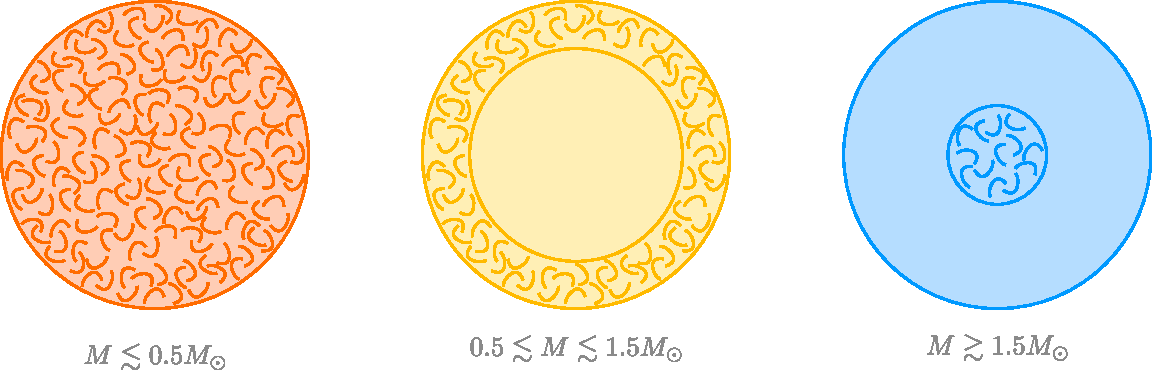
\includegraphics{../assets/10_stellar_evo/convection.pdf}
\caption{Different forms of energy transport in main-sequence stars
according to their masses.}
\end{figure}

As a star evolves in the main sequence it depletes core hydrogen. solar
mass stars and high mass stars show a distinctive difference in their
abundance profiles as they evolve towards core-hydrogen depletion. Low
mass stars exhibit a smooth composition profile with hydrogen mass
fractions having their lowest value at the core, while intermediate and
massive stars have well mixed cores where hydrogen is kept at a nearly
fixed abundance.

\begin{figure}
\centering
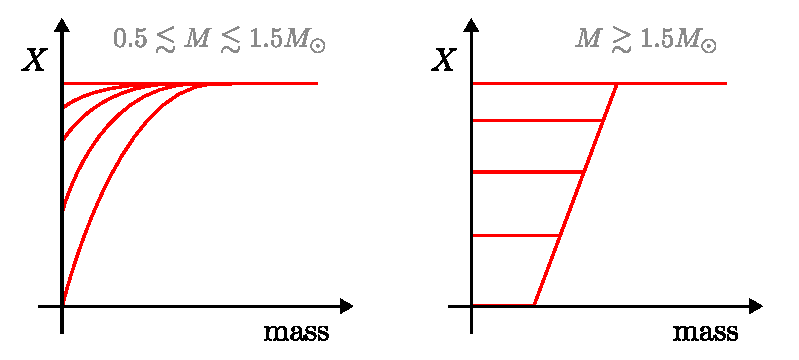
\includegraphics{../assets/10_stellar_evo/composition.pdf}
\caption{Sketch of the evolution of hydrogen mass fraction profiles
through the main-sequence for stars of different masses.}
\end{figure}

As illustrated above, the convective cores of intermediate and massive
stars recede in the mass coordinate as the star evolves. This reduction
of the convective core mass is partially explained by the lowered
opacity of helium rich material. As deep in the stellar interior opacity
is well approximated by electron scattering,
\(\kappa_\mathrm{es}=0.2(1+X)\;\mathrm{cm^2\,g^{-1}}\), and as
\(\nabla_\mathrm{rad}\propto \kappa_\mathrm{es}\) a decrease in \(X\)
decreases \(\nabla_\mathrm{rad}\) favoring convective stability.
Although this is an important element, one needs to be careful with this
argument as \(\nabla_\mathrm{rad}\) depends on various other properties
that do not remain fixed as the star evolves.

\hypertarget{evolution-in-the-rho_mathrmc-t_mathrmc-diagram}{%
\subsection{\texorpdfstring{Evolution in the
\(\rho_\mathrm{c}\)-\(T_\mathrm{c}\)
diagram}{Evolution in the \textbackslash rho\_\textbackslash mathrm\{c\}-T\_\textbackslash mathrm\{c\} diagram}}\label{evolution-in-the-rho_mathrmc-t_mathrmc-diagram}}

Thinking beyond the main sequence we can make use of our results so far
to discuss the conditions under which stars ignote different nuclear
fuels. Before \(H\) is ignited, or in-between burning phases, evolution
can be approximately described by homologous contraction. Beyond the
main sequence the hydrogen envelope can expand significantly, but the
helium core will contract near-homologously. Using our homology
relationships derived in the previous class we find that

\[\rho_\mathrm{c}\propto MR^{-1},\quad \rho_\mathrm{c}\propto MR^{-3}.\]

Since we have

\[R^{-1}\propto T_\mathrm{c}M^{-1},\]

we get

\[\rho_\mathrm{c}\propto M^{-2}T_\mathrm{c}^3\;\rightarrow\; \log T_\mathrm{c} =\frac{2}{3}\log M + \frac{1}{3}\log \rho_\mathrm{c}.\]

This indicates that at the same central density stars of higher mass
have a higher central temperature.

Now, these homology relationships were made using an ideal gas equation
of state but they can break down as we reach higher densities and the
gas potentially becomes degenerate. We can assess this by considering
the characteristic energy of a particle of the ideal gas,

\[E_\mathrm{id} = k_\mathrm{B}T\]

and the energy associated to a particle with the Fermi momentum. In the
non-relativistic case we have

\[R_\mathrm{deg,NR}\sim \frac{p_\mathrm{F}}{2m},\;p_\mathrm{F}\propto \rho^{1/3}\;\rightarrow\;E_\mathrm{deg}\propto\rho^{2/3}.\]

In the extremely relativistic case we have

\[E_\mathrm{deg, ER}\sim p_\mathrm{F}c\propto \rho^{1/3}.\]

Moreover we can determine a critical density of a degenerate gas,
\(\rho_\mathrm{crit}\), above which the ER regime is a more appropriate
description,

\[\frac{E_\mathrm{deg,NR}(\rho_\mathrm{crit})}{E_\mathrm{deg,ER}(\rho_\mathrm{crit})}\sim 1\;\rightarrow \rho_\mathrm{crit}=\mathrm{constant}.\]

This allows us to draw various boundaries in a
\(\log T_\mathrm{c}-\log \rho_\mathrm{c}\) plane, which are sketched
below.

\begin{figure}
\centering
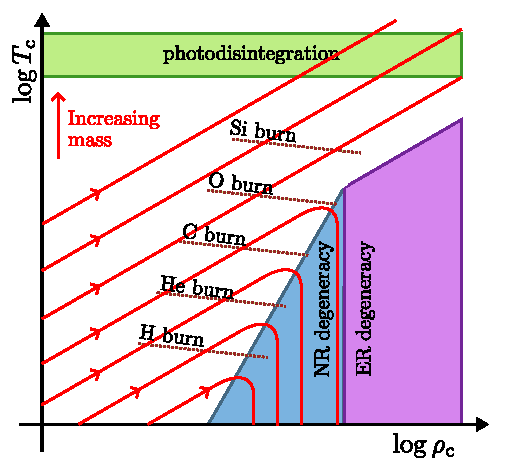
\includegraphics{../assets/10_stellar_evo/log_T_rho.pdf}
\caption{Illustrative evolution of stars in the
$\log\rho_{\mathrm{c}}-\log T_{\mathrm{c}}$ diagram.}
\end{figure}

Red lines illustrate the evolution of stars with different masses, while
the dashed lines show different ignition lines for nuclear fuels. As we
discussed while studying nucleosynthesis, burning stages are well
separated in temperature and have a very strong temperature dependency,
making these lines close to horizontal in the diagram. Stars with lower
masses reach the non-relativistic degeneracy regime at earlier
evolutionary stages, at which point temperature decouples from pressure
and the star stops contracting and cools down. This corresponds to the
white dwarf stage, and more massive stars can produce different types of
white dwarfs (helium, CO and O-Ne-Mg white dwarfs). Stars born with more
than \(\sim 8M_\odot\) avoid the electron degeneracy region, and keep
contracting and heating up beyond silicon burning. Eventually, the
central temperature becomes so high that photons within the gas are
extremely energetic and can destroy nuclei, undoing the chain of fusion
processes that led to an iron-core in an endothermic process that leads
to core-collapse and the formation of a neutron star or black-hole.

It is important to point out two other different outcomes. Stars
slightly below \(8M_\odot\) can undergo collapse of their O-Ne-Mg cores
due to electron captures into Magnesium and Neon, which is expected to
result in a neutron star. Stars that finish their lives with helium
cores in excess of \(\sim 45M_\odot\) (noting there are large
uncertainties on this due to uncertainties in nuclear reaction rates)
are expected to experience an instability due to the creation of
electron positron pairs in their cores, which softens the equation of
state and leads to collapse before oxygen depletion. This produces a
thermonuclear condition which can disrupt the entire star (known as a
pair-instability supernova) leaving no compact remnant behind.

\end{document}
